% 
% Just another Fuel Cell Formulary by Dr. Alexander Kabza
%
% Created: November 4, 2002 (started as Word document, converted to LaTeX in August 2010)
% last modified: 2025-03-19 - this version can be optimized for DIN A4 page layout or Smartphone layout (DIN A5 page layout)!
%
% Open issues: (marked by ***)
% - 
%

% for A4 page layout
\documentclass[11pt,a4paper,english,twoside]{scrreprt}
\usepackage{a4wide}
\usepackage{version}
\includeversion{A4}
\excludeversion{Smartphone}

% for Smartphone page layout
%\documentclass[12pt,a5paper,english,oneside]{scrreprt}
%\usepackage[a5paper, left=1.0cm, right=1.0cm, top=1.5cm, bottom=2.3cm]{geometry}
%\usepackage{version}
%\includeversion{Smartphone}
%\excludeversion{A4}


%%% remove comment delimiter ('%') and specify encoding parameter if required,
%%% see TeX documentation for additional info (cp1252-Western,cp1251-Cyrillic)
%\usepackage[cp1252]{inputenc}

\usepackage[english]{babel}
%\usepackage[html,png]{tex4ht}
%\usepackage{amssymb}
\usepackage{amsmath}
\usepackage{graphicx}
\usepackage{helvet}
\usepackage{parskip}
\usepackage{subcaption}
\usepackage{siunitx}
\usepackage{mhchem}

%\usepackage{lastpage}
\usepackage{wrapfig}
\usepackage[pdfborder=1 1 1]{hyperref}

% for URLs
\usepackage[colorlinks=true,urlcolor=blue,linkcolor=green]{hyperref}

% Alias
\renewcommand{\familydefault}{\sfdefault}
\newcommand{\gradC}{${}^\circ$C}      % fuer Grad Celsius in Text-Umgebung

%\sloppypar

% Kopf- und Fu"szeilendefinition mit fancyhdr-Packet
\usepackage{fancyhdr}
\pagestyle{fancy}
\renewcommand{\chaptermark}[1]{\markboth{\thechapter\ #1}{}}
\renewcommand{\sectionmark}[1]{\markright{\thesection\ #1}{}}
\fancyhead{}
\fancyhead[LO,RE]{\footnotesize \rightmark}
\fancyhead[LE,RO]{\footnotesize \thepage}
\fancyfoot{}
%\fancyfoot[C]{\footnotesize empty}
\fancyfoot[LE,RO]{\footnotesize Fuel Cell Formulary}
\fancyfoot[LO,RE]{\footnotesize \copyright \ Alexander Kabza}
\renewcommand\headrulewidth{1pt}
\renewcommand\footrulewidth{0.5pt}

% die Seite, auf der ein neues chapter beginnt, soll auch Kopf- und Fusszeile bekommen
\fancypagestyle{plain}{%
\renewcommand{\headrulewidth}{1pt}
\renewcommand{\footrulewidth}{0.5pt}}

\AtBeginDocument{\DeclareSIUnit{\kWh}{kWh}}
\AtBeginDocument{\DeclareSIUnit{\normliter}{Nl}}

\begin{document}

\selectlanguage{english}

\title{\Large Just another \\[.75cm] 
  \Huge Fuel Cell Formulary}
\author{\Large by Dr. Alexander Kabza}
\begin{A4}
  \date{
    \scriptsize Created 2001-03-16 -- last updated \today\ and optimized for DIN A4 page layout.
    \\[.3cm] 
    For the latest PDF version visit  \url{www.kabza.de} or
    \url{https://github.com/akabza/Fuel-cell-formulary}
    \\[.3cm]
    Don't hesitate to send me any comments or failures or ideas by email!
    \\[2cm]
    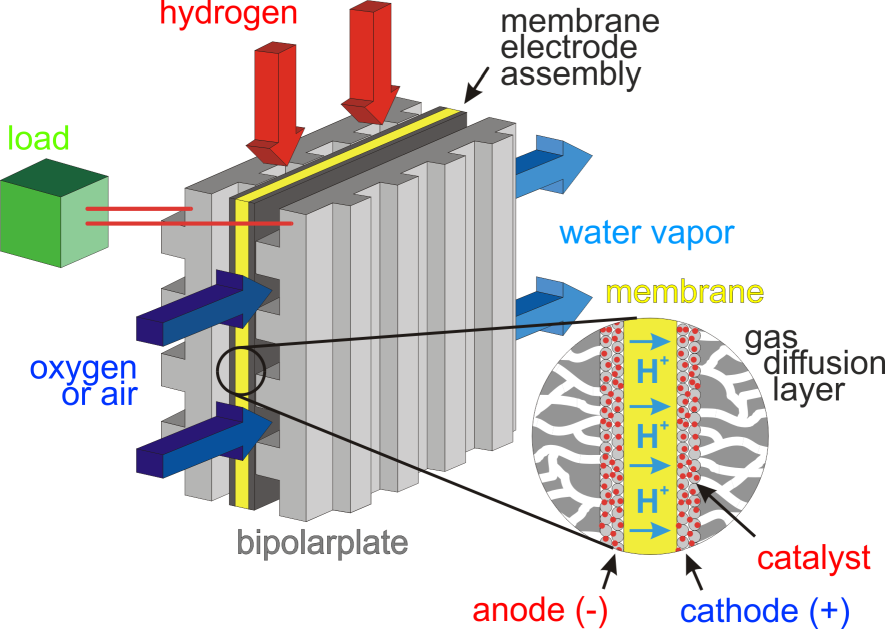
\includegraphics[width=13cm]{PEMFC_EN_small.png}
  }
\end{A4}  
\begin{Smartphone}
  \date{
    \scriptsize Created 2001-03-16.
    \\[.3cm]
    This version is from \today\ and optimized for Smartphones.
    \\[.3cm] 
    For the latest PDF version visit \url{www.kabza.de} or
    \url{https://github.com/akabza/Fuel-cell-formulary}
    \\[.3cm]
    Don't hesitate to send me any comments or failures or ideas by email!
    \\[2cm]
    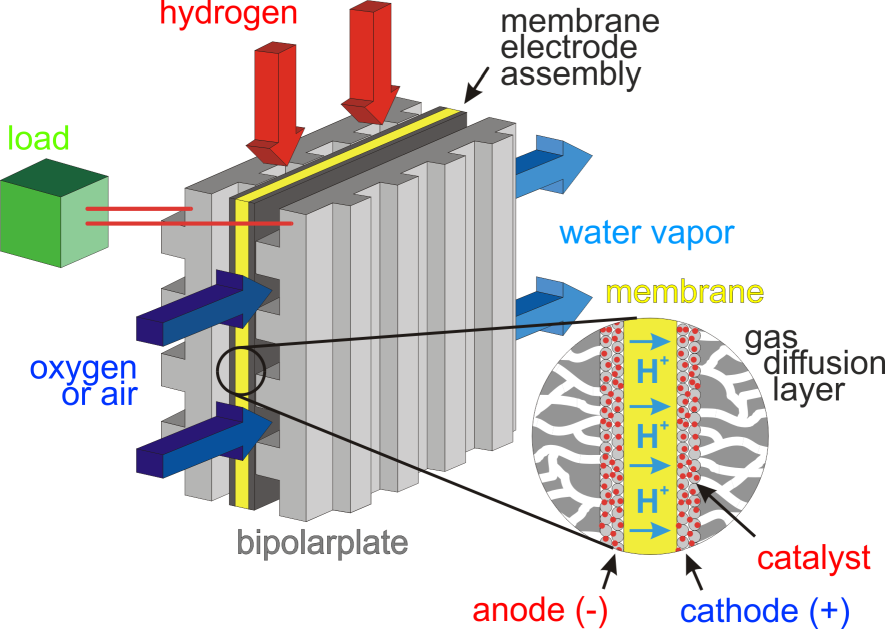
\includegraphics[width=13cm]{PEMFC_EN_small.png}
  }
\end{Smartphone} 
 
\maketitle

\tableofcontents    % Inhaltsverzeichnis


%---------------------
\chapter{Fundamentals}
%---------------------

This is a collection of relevant formulas, calculations and equations for designing a fuel cell system (FCS).


%----------------------------------------------------------------
\section{Thermodynamic of \ce{H2}/\ce{O2} electrochemical device}
%----------------------------------------------------------------

In an \ce{H2}/\ce{O2} electrochemical device hydrogen is oxidized by oxygen to water in an exothermic reaction:

\[\ce{H2} + \frac 12 \ce{O2} \to \ce{H2O}_{(g)} \quad \Delta_r H < 0\]

The \textit{reaction enthalpy} $\Delta_r H$ is equal to the \textit{enthalpy of water formation} $\Delta_f H$. The (chemical) energy content of any fuel is called \textit{heating value} (for more information on thermodynamics see chapter~\ref{sec:Thermodynamics}). The heating value of hydrogen is equal to the absolute value of the reaction enthalpy. Because product water is produced either as gaseous or liquid phase, we distinguish between the \textit{lower heating value} (LHV) and the \textit{higher heating value} (HHV) of hydrogen:

\[\ce{H2} + \frac 12 \ce{O2} \to \ce{H2O}_{(g)} \quad -\Delta_f H_{\ce{H2O}_{(g)} } =\text{LHV}=\SI{241.82}{\kilo\joule\per\mole}\]

\[\ce{H2} + \frac 12 \ce{O2} \to \ce{H2O}_{(l)} \quad -\Delta_f H_{\ce{H2O}_{(l)} } =\text{HHV}=\SI{285.83}{\kilo\joule\per\mole}\]

Please note that LHV and HHV have positive signs whereas $\Delta H$ is negative. All thermodynamic potentials are dependent on temperature and pressure, but are defined at thermodynamic standard conditions ($\SI{25}{\degreeCelsius}$ and $\SI{100}{\kilo\pascal}$, standard ambient temperature and pressure SATP, see also section~\ref{sec:STP}).

The difference between LHV and HHV of $\SI{44.01}{\kilo\joule\per\mole}$ is equal to the molar latent heat of water vaporization at $\SI{25}{\degreeCelsius}$.

The (thermodynamic) \textit{electromotive force (EMF)} or \textit{reversible open cell voltage (OCV)}~$E^{0}$ of any electrochemical device is defined as:

\[E^{0} =\frac{\Delta G}{n\cdot F} \]

where $n$ is the amount of exchanged electrons and $F$ is Faraday's constant (see chapter~\ref{sec:const}). For more information see chapter~\ref{sec:Thermodynamics}. For the hydrogen oxidation or water formation $n=2$. The free enthalpies $\Delta G$ of water formation is either 
\[
\Delta_f G_{\ce{H2O}_{(g)} } =\SI{-228.57}{\kilo\joule\per\mole} \quad \mbox{or} \quad
\Delta_f G_{\ce{H2O}_{(l)} } =\SI{-237.13}{\kilo\joule\per\mole}
\]

Therefore the corresponding EMFs are:
\begin{equation}
  \label{eqn:E_dG}
  E_{g}^{0} =\frac{-\Delta_f G_{\ce{H2O}_{(g)}}}{2F} =\SI{1.184}{\volt} \qquad
  E_{l}^{0} =\frac{-\Delta_f G_{\ce{H2O}_{(l)}}}{2F} =\SI{1.229}{\volt}
\end{equation}

These voltages are the maximum voltages which can (theoretically) be obtained from the electrochemical reaction of \ce{H2} and \ce{O2}. Beside that it make sense to define two other voltages to simplify the efficiency calculations (see section~\ref{sec:Efficiency}). If all the chemical energy of hydrogen (i.e. its heating value) were converted into electric energy (which is obviously not possible!), the following voltage equivalents would result:

\begin{equation}
  \label{eqn:E_dH}
  E_\text{LHV}^{0} =\frac{\text{LHV}}{2F} =\SI{1.253}{\volt} \qquad
  E_\text{HHV}^{0} =\frac{\text{HHV}}{2F} =\SI{1.481}{\volt}
\end{equation}

Those two values are the \textit{voltage equivalent} to the enthalpy $\Delta H$, also called \textit{thermal cell voltage} (see \cite{HFC}, page 27) or \textit{thermoneutral voltage}.

The thermodynamic potentials $\Delta H$ and $\Delta G$ are dependent on temperature; therefore also the corresponding voltage equivalents are functions of temperature. The temperature dependency (of absolute values) is shown in figure \ref{fig:DG_DH}, values are calculated with HSC Chemistry 6.21. 

\begin{figure}
  \centering
  \includegraphics*[width=0.9\textwidth,angle=0]{FCF_Table_LHV_HHV.pdf}  
  \includegraphics*[width=0.7\textwidth,angle=0]{FCF_Chart_LHV_HHV.pdf}  
  \caption[$\Delta H$ and $\Delta G$ as a function of temperature]{$\Delta H$ and $\Delta G$ as a function of temperature}
  \label{fig:DG_DH}
\end{figure}


%------------------------
\section{Nernst equation}
%------------------------

The theoretical cell porential or electromotive force (EMF) is not only depending on the temperatue (as shwon in the previous section), but also depending on the pressure. This dependency is in general described by the Nernst equation. For the \ce{H2}/\ce{O2} electrochemical reaction the Nernst equation is:

\begin{equation}
	\label{eq:Nernst}
	E = E^{0} + \frac{RT}{2F} \ln \left(\frac{p_{\ce{H2}} p^{1/2}_{\ce{O2}}}{p_{\ce{H2O}}} \right)  
\end{equation}

$p$ is the partial pressure of \ce{H2}, \ce{O2} and \ce{H2O}.

Introducing a system pressure $p_{\text{Sys}}$ and defining $p_{\ce{H2}} = \alpha\, p_{\text{Sys}}$, $p_{\ce{O2}} = \beta\, p_{\text{Sys}}$, $p_{\ce{H2O}} = \gamma\, p_{\text{Sys}}$, the Nernst equation simplifies to:

\begin{equation}
	\label{eq:Nernst2}
	E = E^{0} + \frac{RT}{2F} \ln \left(\frac{\alpha \beta^{1/2}}{\gamma}\right) + \frac{RT}{4F} \ln p_{\text{Sys}}   
\end{equation}

If $\alpha$, $\beta$ and $\gamma$ are constant, increasing the system pressure from $p_1$ to $p_2$ influences the cell potential as follows:

\begin{equation}
	\label{eq:Nernst3}
	\Delta E = \frac{RT}{4F} \ln \frac{p_2}{p_1}   
\end{equation}

Assuming a cell runs at $\SI{80}{\degreeCelsius}$, then doubling the system pressure results in a potential increase of $\Delta E = \SI{7.6}{\milli\volt} \ln 2 = \SI{5.27}{\milli\volt}$. It is important to mention that due to other effects an increase in system pressure results in much higher cell voltage increas than just given by Nernst equation!




%--------------------------------------
\section{Reactant consumption and feed}
%--------------------------------------

The reactants \ce{H2} and \ce{O2} are consumed inside the fuel cell stack by the electrochemical reaction. Based on the \textit{Faraday's laws} the molar flows $\dot{n}$ for reactant consumptions are defined as follows:

\begin{equation}
  \label{eqn:n_H2_consumed}
  \dot{n}_{\ce{H2}} = \frac{I\cdot N}{2F} \qquad [\dot{n}_{\ce{H2}}]=\si{\mole\per\second}
\end{equation}

\[\dot n_{\ce{O2}} =\frac{I\cdot N}{4F} =\frac 12 \cdot \dot{n}_{\ce{H2}} \qquad [\dot{n}_{\ce{O2}}]=\si{\mole\per\second}\]

$I$ is the stack load (electric current, $[I]=A$), and $N$ is the amount of single cells (cell count, $[N]=-$). 2 is again the amount of exchanged electrons per mole \ce{H2} for the hydrogen oxidation; respectively 4~e\textsuperscript{-} per mole \ce{O2} for the oxygen reduction reaction. $F$ is the Faraday constant.

The stoichiometry $\lambda$ defines the ratio between reactant feed (into the fuel cell) and reactant consumption (inside the fuel cell). Due to fuel cell design and water management issues etc. the stoichiometry must always be more than one:

\[\lambda =\frac{\dot{n}_{\text{feed}}}{\dot{n}_{\text{consumed}}} > 1 \qquad [\lambda] = -\]


The reactant feed for \ce{H2} and air into the fuel cell stack are now defined by an anode and cathode stoichiometry~$\lambda$:

\begin{equation}
  \label{eqn:n_H2_feed}
  \dot n_{\ce{H2},\,\text{feed}} = \dot n_{\ce{H2}} \cdot \lambda_{\text{anode}} = \frac{I\cdot N}{2F} \cdot \lambda _{\text{anode}}
\end{equation}

\[
\dot n_{\text{air,\,feed}} = \frac{\dot n_{\ce{O2}}}{x_{\ce{O2}}} \cdot \lambda _{\text{cathode}}= \frac{I\cdot N}{4F\cdot x_{\ce{O2}}} \cdot \lambda _{\text{cathode}}
\]

where $x_{\ce{O2}}$ is the oxygen content in air.



The molar flows of unconverted (dry) reactants at the stack exhaust are given as:

\[\dot{n}_{\ce{H2},\,\text{out}} =\dot{n}_{\ce{H2},\,\text{feed}} -\dot{n}_{\ce{H2}} =\frac{I\cdot N}{2F} \cdot (\lambda_{\text{anode}} -1)\]

\[\dot{n}_{\text{air,\,out}} =\dot{n}_{\text{air,\,feed}} -\dot{n}_{\ce{O2}} =\frac{I\cdot N}{4F} \cdot \left(\frac{\lambda_{\text{cathode}} }{x_{\ce{O2}}} -1\right)\]


It is very common to give the reactant feed either as a mass or volume flow. The mass flow $\dot{m}$ is the product of molar flow $\dot{n}$ and molar weight $M$:

\[\dot{m}=\dot{n} \cdot M \qquad [\dot{m}]=\si{\gram\per\second}\]

The mass flow for stack anode and cathode inlet are therefore:

\begin{equation}
  \label{eqn:mdot_H2_feed}
  \dot m_{\ce{H2},\,\text{feed}} = \frac{I N}{2 F} \cdot \lambda_{\text{anode}} \cdot M_{\ce{H2}}
\end{equation}

\begin{equation}
  \label{eqn:mdot_air_feed}
  \dot m_{\text{air,\,feed}} = \frac{I N}{4 F x_{\ce{O2}}} \cdot \lambda_{\text{cathode}} \cdot M_{\text{air}}
\end{equation}

The dry mass gas flow at stack cathode outlet contains less oxygen than air and is calculated as:

\begin{equation}
  \label{eqn:mdot_cathode_feed}
  \dot m_{\text{cathode,\,out}} = \dot m_{\text{air,\,feed}} - \dot m_{\ce{O2},\,\text{consumed}} =
  \frac{I N}{4 F} \cdot \left(\frac{\lambda_{\text{cathode}}}{x_{\ce{O2}}} \cdot M_{\text{air}} - M_{\ce{O2}}\right)
\end{equation}

The volume flow $\dot{V}$ is calculated by the gas density $\rho$ or the molar gas volume $V_{\text{0,\,mol}}$:

\[\dot{V}=\frac{\dot{m}}{\rho}=V_{\text{0,\,mol}} \cdot \dot{n} \qquad [\dot{V}]=\si{\liter\per\minute} \]


Both the gas density $\rho$ and the molar gas volume $V_{\text{0,\,mol}}$ are temperature and pressure dependent! Therefor the referring temperature and pressure need to be defined. $N$ or $n$ indicates that the volume flow is normalized to a specific reference temperature and pressure (e.g. $[\dot{V}]=\text{Nl/min}$ or $\text{l}_{\text{n}}\text{/min}$). Physical standard temperature and pressure (STP) is defined as $\SI{0}{\degreeCelsius}$ and $\SI{101.325}{\kilo\pascal}$ (for more information see section~\ref{sec:STP}). The molar gas volume at STP is $V_{\text{0,\,mol}}=\SI{22.414}{\normliter\per\mole}$.

The amount of product water is equal to hydrogen consumption (equation~\ref{eqn:n_H2_consumed}) and given by:

\[\dot n_{\ce{H2O},\,\text{prod}} = \dot n_{\ce{H2}} = \frac{I\cdot N}{2F} \qquad [\dot n_{\ce{H2O}}]=\si{\mole\per\second} \]

The product water mass flow is:

\begin{equation}
  \label{eqn:mdot_water}
  \dot m_{\ce{H2O},\,\text{prod}} = \frac{I\cdot N}{2F} \cdot M_{\ce{H2O}} \qquad [\dot m_{\ce{H2O}}]=\si{\gram\per\second}
\end{equation}


%----------------------------------
\section{Hydrogen energy and power}
\label{sec:HyEnergyPower}
%----------------------------------

Hydrogen is a chemical energy carrier with a specific (chemical) energy density, which is defined by either HHV or LHV. The {\em mass} specific chemical energy is:

\[W_{\ce{H2},\,\text{HHV}} =\frac{\text{HHV}}{M_{\ce{H2}}} = \frac{\SI{285.83}{\kilo\joule\per\mole}}{\SI{2.02}{\gram\per\mole}} = \SI{141.79}{\kilo\joule\per\gram} \equiv \SI[sticky-per]{39.39}{\kWh\per\kilo\gram}\]

\[W_{\ce{H2},\,\text{LHV}} =\frac{\text{LHV}}{M_{\ce{H2}}} = \frac{\SI{241.82}{\kilo\joule\per\mole}}{\SI{2.02}{\gram\per\mole}} = \SI{119.96}{\kilo\joule\per\gram} \equiv \SI[sticky-per]{33.32}{\kWh\per\kilo\gram}\]

The {\em volume} specific chemical energy (at STP) is:

\[W_{\ce{H2},\,\text{HHV}} =\frac{\text{HHV}}{M_{\ce{H2}}} = \frac{\SI{285.83}{\kilo\joule\per\mole}}{\SI{22.414}{\normliter\per\mole}} = \SI{12.75}{\kilo\joule\per\liter} \equiv \SI[sticky-per]{3.54}{\kWh\per\cubic\meter}\]

\[W_{\ce{H2},\,\text{HHV}} =\frac{\text{HHV}}{M_{\ce{H2}}} = \frac{\SI{285.83}{\kilo\joule\per\mole}}{\SI{22.414}{\normliter\per\mole}} = \SI{10.79}{\kilo\joule\per\liter} \equiv \SI[sticky-per]{3.00}{\kWh\per\cubic\meter}\]

The chemical power of an \ce{H2} flow is:

\begin{equation}
  \label{eqn:P_H2_flow}
  P_{\ce{H2},\,\text{HHV}} = {\text{HHV}} \cdot \dot{n}_{\ce{H2}} \qquad 
  P_{\ce{H2},\,\text{LHV}} = {\text{LHV}} \cdot \dot{n}_{\ce{H2}} \qquad [P_{\ce{H2}}]=\si{\joule\per\second}=\si{\watt} 
\end{equation}


\[ = 212.5\frac{\si{W}}{\si{\normliter\per\minute}}  \qquad = 179.8\frac{\si{W}}{\si{\normliter\per\minute}} \]



Now the (chemical) power of \ce{H2} consumed in a stack (with $N$ cells at the stack load $I$) using equations~\ref{eqn:E_dH} and \ref{eqn:n_H2_consumed} can easily be expressed as:

\begin{equation}
  \label{eqn:P_H2_consumed}
  P_{\ce{H2},\,\text{HHV\,consumed}} = \SI{1.481}{\volt} \cdot N \cdot I 
\end{equation}


And accordingly the (chemical) power of \ce{H2} feed with equations~\ref{eqn:E_dH} and \ref{eqn:n_H2_feed} is:

\begin{equation}
  \label{eqn:P_H2_feed}
  P_{\ce{H2},\,\text{HHV\,feed}} = \SI{1.481}{\volt} \cdot N \cdot I \cdot \lambda_{\text{anode}}
\end{equation}



%----------------------------------------------
\section{PolCurve (Current voltage dependency)}
\label{sec:polcurve}
%----------------------------------------------

The current voltage dependency of a fuel cell is the most important property to express the performance of a fuel cell. This dependency is nonlinear due to kinetics of the electrochemical reaction of hydrogen and oxygen; it's called current voltage curve (I-U curve) or polarization curve (PolCurve) or performance characteristic. 

%-----------------------------------------------------------------
\subsection{Kinetic of the \ce{H2}/\ce{O2} electrochemical device}
%-----------------------------------------------------------------

The kinetics of electrochemical reaction is relevant as soon as the electric circuit of any electrochemical device is closed and it starts providing electric power. As soon as electrons and ions start moving we get voltage losses (overvoltage). This voltage losses are nonlinear functions of the load (or current density).

Voltage losses are the result of
\begin{itemize}
	\item Oxygen reduction reaction (ORR) kinetics,
	\item Ohmic losses due to membrane ionic conductivity,
	\item Mass transport limitations at high load and
	\item Hydrogen oxidation reaction (HOR) kinetics (less relevant).
\end{itemize}



%----------------------------------
\subsection{Butler-Volmer equation}
\label{sec:ButlerVolmer}
%----------------------------------

The kinetics of ORR can be described with the Butler-Volmer equation. The Butler-Volmer equation defines the relation between current density $j$ and overpotential $\varphi$ of any electrochemical reaction:

\[
j(\varphi) = j_0 \left[\exp\left(\frac{\alpha n F}{RT}\: \varphi \right) - \exp\left(\frac{-(1-\alpha) n F}{RT}\: \varphi \right) \right]
\]

This is the sum of an anodic and cathodic current $j(\varphi) = j_a(\varphi) + j_c(\varphi)$ with:

\[
j_a(\varphi) = j_0 \exp\left(\frac{\alpha n F}{RT}\: \varphi \right) \ \ \
j_c(\varphi) = - j_0 \exp\left(\frac{-(1-\alpha) n F}{RT}\: \varphi \right)
\]

Side information: $e^x - e^{-x} = 2 \sinh x$

With $\alpha = 1/2$ the Butler-Volmer equation can be simplified to:

\[
\frac{j(\varphi)}{j_0} = 2 \sinh \left( \frac12 \frac{n F}{RT}\: \varphi \right) 
\]

\begin{figure}
  \centering
  \begin{subfigure}{.5\textwidth}
    \centering
    \includegraphics*[width=.95\linewidth, angle=0]{FCF_Chart_ButlerVolmer1.pdf}
    \caption{Large overpotential}
    \label{fig:ButlerVolmer1}
  \end{subfigure}%
  \begin{subfigure}{.5\textwidth}
    \centering
    \includegraphics*[width=.95\linewidth, angle=0]{FCF_Chart_ButlerVolmer2.pdf}
    \caption{Small overpotential}
    \label{fig:ButlerVolmer2}
  \end{subfigure}
  \caption[Butler Volmer]{Butler Volmer}
\end{figure}
 
Figure \ref{fig:ButlerVolmer1} shows the anodic current (green line), the cathodic current (blue) and the Butler-Volmer equation itself (red). In case of low overpotentials ($\left|\varphi\right| < \SI{10}{\milli\volt}$, $\alpha = 1/2$) the Butler-Volmer equation simplifies to:

\[
\frac{j(\varphi)}{j_0} = \frac{n F}{RT}\: \varphi 
\]


\begin{figure}  
  \centering
  \includegraphics*[width=0.5\textwidth,angle=0]{FCF_Chart_ButlerVolmer3.pdf}
  \caption[Butler Volmer logarithmic scale]{Butler Volmer logarithmic scale}
  \label{fig:ButlerVolmerLog}
\end{figure}

Figure \ref{fig:ButlerVolmer2} shows this linear relation between current density $j$ and overpotential $\varphi$, with the slope $m=nF/RT$. In case of high overpotentials ($\left|\varphi\right| > \SI{100}{\milli\volt}$, $\alpha = 1/2$) the Butler-Volmer equation simplifies to:

\[
\ln \frac{j(\varphi)}{j_0} = \frac12 \frac{n F}{RT}\: \varphi 
\]

This relation becomes linear by using a logarithmic y-axes like shown in figure \ref{fig:ButlerVolmerLog}. The slope of the blue dotted line $m=1/2\ nF/RT$ is the Tafel slope in the Tafel equation $\varphi = m \cdot j/j_0$. 



%----------------------------
\subsection{Example PolCurve}
%----------------------------

The PolCurve plots the cell voltage versus current density of a single cell or stack. Figure \ref{fig:PolCurve} shows an theoretical PolCurve, including the electric and thermal power based on LHV or HHV (equation~\ref{eqn:P_therm}), and the electric efficiency based on LHV (\ref{eqn:eta_el}).

\begin{figure}
  \centering
  \includegraphics*[width=0.9\textwidth,angle=0]{FCF_Chart_PolCurve.pdf}
  \caption[Polarization curve]{Polarization curve}
  \label{fig:PolCurve}
\end{figure}

For simulation and modeling it is helpful to have a mathematical expression for the PolCurves. The following empirical equation with physical background describes the 
voltage current dependency quite well (see \cite{lit:Srinivasan}, \cite{lit:Kim}):

\begin{equation}
  \label{eqn:E_empirical}
  E = E_0 - b \cdot (\log j +3) - R j - m \cdot e^{n j}
\end{equation}

The parameters are:
\begin{itemize}
	\item $E_0$: (measured) open cell voltage, $[E_0]=\si{\volt}$
	\item $j$: Current density, $[j]=\text{A/cm}^{\text{2}}$
	\item $b$: Tafel slope (voltage drop due to oxygen reduction reaction), $[b]=\text{V/dec}$
	\item $R$: Internal resistor, $[R]=\Omega\,\text{cm}^{\text{2}}$
	\item $m$, $n$: (Empirical) coefficients defining the voltage drop due to diffusion limitation, $[m]=\si{\volt}$, $[n]=\text{cm}^\text{2}/\text{A}$

\end{itemize}

The example PolCurve in the chart \ref{fig:PolCurve} is calculated with the following parameters: $E_0=1.0\,\mathrm{V}$, $b=0.08\,\mathrm{V/dec}$, $R=0.1\,\Omega\,cm^2$, $m=0.0003\,\mathrm{V}$, and $n=3.30\,\mathrm{cm^2/A}$.



%------------------------------
\section{Fuel cell stack power}
%------------------------------


\paragraph{Electric stack power}

$P_{\text{el}}$ is the product of stack voltage and stack load, also called \textit{gross} power:

\begin{equation}
  \label{eqn:P_gross}
   P_{\text{el}} =U_{\text{Stack}} \cdot I = \text{AveCell} \cdot N \cdot I
\end{equation}

where $\text{AveCell} = U_{\text{Stack}} / N$ is the average single cell voltage.


\paragraph{Thermal stack power}

$P_{\text{therm}}$ is that part of the consumed chemical fuel power which is \textit{not} converted into electric power:

\[
	P_{\text{therm}} = P_{\ce{H2},\,\text{HHV}} - P_{\text{el}}
\]

For the hydrogen fuel cell it is defined based on HHV as:

\begin{equation}
  \label{eqn:P_therm}
  P_{\text{therm,\,HHV}} =\left(\SI{1.481}{\volt} - {\text{AveCell}}\right) \cdot N \cdot I = P_{\text{el}} \left(\frac{\SI{1.481}{\volt}}{\text{AveCell}} - 1\right)
\end{equation}

The voltage equivalent $\SI{1.481}{\volt}$ is defined by equation~\ref{eqn:E_dH}. To calculate the thermal power based on LHV this voltage equivalent needs to be replaced by $\SI{1.253}{\volt}$.


\paragraph{Recovered heat}

The recovered heat is that part of the thermal stack power that is actually converted into usable heat. This is e.g. the heat transferred into the (liquid) coolant and can be calculated as follows:

\[
	P_{\text{recovered\; heat}} =\dot{V}\cdot c_{p} \cdot \Delta T\cdot \rho
\]

Coolant parameters are: Volume flow $\dot{V}$, heat capacity $c_{p}$, temperature increase $\Delta T$ and density $\rho$.


Due to technical issues not all thermal power can be transferred to coolant; therefore:

\[
	P_{\text{recovered\;heat}} < P_{\text{therm,\,HHV}} 
\]


The unusable or waste heat:

\[
	P_{\text{waste\;heat}} =P_{\text{therm,\,HHV}} -P_{\text{recovered\;heat}} 
\]


This waste heat consists of two parts:

\begin{enumerate}
\item  Heat rejected to ambient via stack surface (radiant heat).
\item  Heat loss by cathode exhaust enthalpy; or more precise by the difference between air outlet and air inlet enthalpy.
\end{enumerate}


%-------------------------------
\section{Fuel cell efficiencies}
\label{sec:Efficiency}
%-------------------------------

\subsection{Different efficiencies}

There seems to be no commitment how to define or name the different efficiencies for fuel cells. Therefore the only thing I can do here is to clarify the differences; well knowing that in literature other definitions and wordings are used. \textit{Don't talk about efficiency if you don't know what you are talking about!}

All efficiencies can be based on either LHV or HHV of the fuel. There is also no commitment to use LHV or HHV. Therefore be careful and keep in mind that the efficiency is higher if it refers to LHV!

In general the energy conversion efficiency $\eta$ is defined as:
\[
	\eta=\frac{\text{(useful)~energy~output}}{\text{energy~input}} = \frac{\text{(useful)~power~output}}{\text{power~input}}
\]

\paragraph{Thermodynamic efficiency}

The thermodynamic or \textit{maximum} or \textit{ideal} efficiency is the ratio between enthalpy (or heating value) $\Delta H$ and Gibbs free enthalpy $\Delta G$ (reflecting the maximum extractible work) of any electrochemical device:

\[
	\eta _{\text{el,\,max}} =\frac{\Delta G}{\Delta H}
\]


For the hydrogen fuel cell it is:

\[
	\eta _{\text{el,\,TD,\,LHV}} =\frac{-\Delta_f G_{\ce{H2O_{(g)}}}}{\text{LHV}} =\frac{E_{g}^{0} }{E_\text{LHV}^{0} } = 
	\frac{\SI{1.184}{\volt}}{\SI{1.253}{\volt}} = \SI{94.5}{\percent}%
\]

\[
	\eta _{\text{el,\,TD,\,HHV}} =\frac{-\Delta_f G_{\ce{H2O_{(l)}}}}{\text{HHV}} =\frac{E_{l}^{0} }{E_\text{HHV}^{0} } = 
	\frac{\SI{1.229}{\volt}}{\SI{1.481}{\volt}} = \SI{83.1}{\percent}%
\]

The Handbook of Fuel Cells \cite{HFC} calls this simply ''ideal efficiency''.

The Fuel Cell Handbook \cite{FCHB} calls this efficiency the ''thermal efficiency of an ideal fuel cell operating \textit{reversibly} on pure hydrogen and oxygen at standard conditions''.

Fuel Cell Systems Explained \cite{FCSE} calls this efficiency ``the maximum efficiency possible'' or ``maximum efficiency limit'' which explains it also very well.


\paragraph{Electric efficiency}

The electric efficiency of a fuel cell (stack) is defined as:

\[
	\eta _{\text{el}} =\frac{P_{\text{el}} }{P_{\text{fuel,\,consumed}}} 
\]

$P_{\text{el}}$ is the stack electric (gross) power and $P_{\text{fuel,\,consumed}}$ is the consumed fuel power (see equations \ref{eqn:P_gross} and \ref{eqn:P_H2_consumed}).

The electric efficiency can easily expressed as (more details see section~\ref{sec:ElEffCalc}):

\begin{equation}
  \label{eqn:eta_el}
   \eta _{\text{el,\,LHV}} = \frac{\text{AveCell}}{\SI{1.253}{\volt}} \quad \mbox{or} \quad
   \eta _{\text{el,\,HHV}} = \frac{\text{AveCell}}{\SI{1.481}{\volt}}
\end{equation}


How this efficiency is named in literature and codes \& standards:

\begin{enumerate}
\item  ``Load efficiency'' in the Handbook of Fuel Cells \cite {HFC}, refers to both LHV and HHV.

\item  The Fuel Cell Handbook \cite{FCHB} refers to HHV and says ``this efficiency is also referred to as the \textit{voltage efficiency}''.

\item  ``Cell efficiency'' in Fuel Cell Systems Explained \cite{FCSE}, and refers to LHV.

\item  SAE J2617 \cite{SAEJ2617} calls this efficiency ``stack sub-system efficiency'' and refers to LHV.
\end{enumerate}


\paragraph{Fuel electric efficiency}

The fuel efficiency considers the amount of hydrogen feed to the stack (and not only the amount of consumed hydrogen). It is defined as:
\[
	\eta _{\text{fuel,\,el}} =\frac{P_{\text{el}}}{P_{\text{fuel,\,feed}}} 
\]

$P_{\text{el}}$ is the stack electric gross power and $P_{\text{fuel,\,feed}}$ is the fuel feed power (see equations \ref{eqn:P_gross} and \ref{eqn:P_H2_feed}).

According to equation~\ref{eqn:eta_el} it is:

\[
  \eta _{\text{fuel,\,el,\,LHV}} = \frac{\text{AveCell}}{\SI{1.253}{\volt} \cdot \lambda_{\text{anode}}} \quad \mbox{or} \quad
  \eta _{\text{fuel,\,el,\,HHV}} = \frac{\text{AveCell}}{\SI{1.481}{\volt} \cdot \lambda_{\text{anode}}}
\]

Obviously, the relation between $\eta_{\text{fuel,\,el}}$ and $\eta_{\text{el}}$ is the anode stoic:

\[
	\eta_{\text{fuel,\,el}} = \frac{\eta_{\text{el}}}{\lambda_{\text{anode}}}
\]


How this efficiency is named in literature:

\begin{enumerate}
\item  Fuel~Cell~Systems~Explained \cite{FCSE} calls this efficiency simply ``efficiency'' (of either LHV or HHV).

\item  Fuel~Cell~Handbook \cite{FCHB} calls it ``\textit{net} cell efficiency`` and defines it as following: ``To arrive at the \textit{net} cell efficiency, the \textit{voltage efficiency} must be multiplied by the fuel utilization.''
\end{enumerate}


\paragraph{Voltage efficiency}

is the ratio between average and reversible cell voltage $E^0$ (see equation~\ref{eqn:E_dG}):

\[
	\eta_{\text{voltage}} =\frac{\text{AveCell}}{E^0} 
\]

Normally the voltage efficiency is based on $\Delta_f G_{\ce{H2O}_{(l)}}$:

\[
	\eta_{\text{voltage}} =\frac{\text{AveCell}}{E_{l}^{0} } = \frac{\text{AveCell}}{\SI{1.229}{\volt}}
\]

\[
	\eta_{\text{voltage}} = \eta_{\text{el,\,HHV}} \cdot \eta_{\text{el,\,TD,\, HHV}}
	= \frac{\text{AveCell}}{\SI{1.481}{\volt}} \cdot \SI{83.1}{\percent}
\]



\paragraph{Thermal efficiency}

$\eta_{\text{therm}}$ can be calculated according the electric efficiency:

\[
	\eta_{\text{therm}} = \frac{P_{\text{therm}}}{P_{\text{fuel,\,consumed}}} 
\]


Based on HHV it is:

\[
	\eta_{\text{therm,\,HHV}} = \frac{\SI{1.481}{\volt} - \text{AveCell}}{\SI{1.481}{\volt}} 
\]



\paragraph{Recovered heat efficiency}

Due to the fact that not all thermal power $P_{\text{therm}}$ is transferred into the coolant the recovery heat efficiency can be calculated:

\[
	\eta_{\text{recovered\;heat}} = \frac{P_{\text{recovered\;heat}}}{P_{\text{therm}}} 
\]


For HHV this is:

\[
  \eta_{\text{recovered\;heat,\;HHV}} = \frac{P_{\text{recovered\;heat}}}{P_{\text{therm,\,HHV}}} 
	= \frac{\dot{V}\cdot c_{p} \cdot \Delta T\cdot \rho }{(\SI{1.481}{\volt} - \text{AveCell}) \cdot N \cdot I} 
\]



\paragraph{Overall stack efficiency}

can be calculated as:

\[
	\eta_\text{overall} = \frac{P_\text{el} + P_\text{therm}}{P_\text{fuel,\,consumed}} = 1 
\]

This (thermodynamic) efficiency needs to be $\eta_\text{overall}=1$, because the consumed hydrogen is converted completely in electric and thermal power:

\[
	P_\text{fuel,\,consumed} = P_\text{el} + P_\text{therm} 
\]


Therefore it is also:

\[
	\eta_\text{overall} = \eta_\text{el} + \eta_\text{therm}
\]


\paragraph{Total efficiency}

is maybe more reasonable and defined as:

\[
	\eta_\text{total} = \frac{P_\text{el} + P_\text{recovered\;heat}}{P_\text{fuel,\,feed}} < 1
\]


Obviously $\eta_\text{total} < 1$, because $P_\text{recovered\;heat} < P_\text{therm}$ and $P_\text{fuel,\,feed} > P_\text{fuel,\,consumed}$!


\subsection{Electric efficiency calculation}
\label{sec:ElEffCalc}

How to convert $\eta_\text{el,\,LHV} = \frac{P_\text{el}}{P_\text{fuel,\,consumed}}$ to $\frac{\text{AveCell}}{\SI{1.253}{\volt}}$?

With equations~\ref{eqn:E_dH} and \ref{eqn:n_H2_consumed} it is:

\[
\begin{array}{lcl}
	\eta_\text{el,\,LHV} &=& \frac{P_\text{el}}{P_\text{fuel,\,consumed}} \\
	&=& \frac{\text{AveCell}\cdot N\cdot I}{\dot{n}_{\ce{H2}} \cdot \text{LHV}} = \frac{\text{AveCell}\cdot 2F}{\text{LHV}} \\
	&=& \frac{\text{AveCell}}{E_\text{LHV}^{0}} = \frac{\text{AveCell}}{\SI{1.253}{\volt}} 
\end{array}
\]


%-------------------------------
\chapter{Fuel cell system (FCS)}
%-------------------------------

IEC 62282-1:2005 \cite{IEC62282-1} defines the main components of a fuel cell system and draws the system boundary around, see figure \ref{fig:FCSbound}. 

\begin{figure}
  \centering
  \includegraphics*[width=0.9\textwidth,angle=0]{FCF_Figure_FCS_boundaries.pdf}
  \caption[Fuel Cell System according to IEC 62282-1]{Fuel Cell System according to IEC 62282-1}
  \label{fig:FCSbound}
\end{figure}

The main components are the fuel cell stack, an air processing system (e.~g. a compressor and humidifier), the fuel gas supply, thermal management system etc. Other peripheral components are valves, pumps, electrical devices etc. Fuel like hydrogen (from a tank system) and air (ambient) are feed into the FCS.

Main FCS inputs are fuel (e.g. hydrogen), air and water, but also electric and thermal power. Main FCS outputs are the electric net and thermal power, the reactant exhaust gases and product water. The (electric) gross power is the stack electric power. The difference between gross and net is the electric power consumed by the peripheral electric components inside the FCS:

\[P_\text{net} =P_\text{gross} -P_\text{paripheral}\]


%------------------------
\section{Anode subsystem}
%------------------------

Hydrogen is feed into the fuel cell system from a tank system. The consumed hydrogen inside the fuel cell stack is based on the Faraday equation (equation~\ref{eqn:n_H2_consumed}) and dependent on the stack load. Actually always more hydrogen is feed into the FCS than is consumed inside the stack. 

The anode flow shall on one hand be high enough to remove product water, but shall on the other hand be low to increase efficiency. This dilemma is often solved by an anode recirculation loop (see figure \ref{fig:AnodeLoop}). 

\begin{wrapfigure}{r}{0.4\textwidth}
  \centering
  \includegraphics*[width=0.4\textwidth,angle=0]{FCF_Figure_Anode_loop.pdf}
  \caption[Anode loop]{Anode loop}
  \label{fig:AnodeLoop}
\end{wrapfigure}  

The anode recirculation is either realized with an Anode Recirculation Pump (ARP) or by one or more jet pumps. A water trapp shall remove liquid water at the anode exhaust. The purge valve opens with a specific frequency and duration to remove inert gases accumulated in the anode loop (mainly nitrogen from the cathode side). The anode loop ensures a high anode gas flow (e.g. $\lambda_\text{gross}>2$) through the stack and allows a nearly complete utilization of hydrogen ($\lambda_\text{net} \ll 1.1$). This stack anode off gas is finally purged either into the cathode exhaust or directly out of the FCS. This purged hydrogen is obviously lost for the electrochemical conversion, therefore the amount of anode purge losses shall be minimized.

The relation between hydrogen feed versus consumed hydrogen is called FCS fuel stoichiometry:

\[
	\lambda_\text{net}=\lambda_\text{fuel, FCS} = \frac{\text{fuel\;feed}}{\text{fuel\;consumed}} = \frac{\ce{H2}\text{feed}}{\ce{H2}\text{consumed}} \ge 1
\]

The fuel efficiency (or fuel utilization) of a FCS is defined as:

\[\eta_\text{fuel, FCS} = 1/\lambda_\text{fuel, FCS} \]

The anode recirculation loop and its anode purge controls needs to be optimized regarding high fuel efficiency or low fuel losses. By doing this the fuel stoichiometry can be close to 1. One controls concept is the Amperehour counter. The anode purge is triggered when the integral of stack load reaches an Ah-threshold of e.g. 50\,Ah. If the stack runs at 300\,A constant load there is one purge every 10\,min, calculated as following:

\[
\frac{\SI{300}{\ampere}}{\SI{50}{\ampere\hour}} = \frac{\SI{300}{\ampere}}{\SI{180,000}{\ampere\second}} = \SI{0.00166}{\per\second} = \SI{0.1}{\per\minute}
\]


%--------------------------
\section{Cathode subsystem}
%--------------------------

An air processing system or cathode submodule is e.g. a compressor and a gas-to-gas humidifier. Its purpose is to feed the conditioned (humidified) and required amount of air into the stack.

Ambient air has a specific relative humidity. Depending on the FCS design, this water input into the FCS may be neglected. More important is the pressure drop inside the stack and inside the FCS, and therefore the absolute pressure after the compressor and before the stack. The cathode stoichiometry is dependent on the system power level; typical values are between 1.8 (at higher load) to 3 (or more at low load).


%-------------------------------------
\subsection{Cathode pressure controls}
%-------------------------------------

In case of (low temperature) PEM fuel cell stacks it is essential to remove all product water from the stack. The stack operating conditions to fulfill this requirement can be calculated. Due to the fact that most water is removed via cathode exhaust; therefore we assume no water removal through anode exhaust. Based on this assumption we get the following equation to calculate the specific humidity at cathode exhaust (more details see chapter \ref{chap:Fuel cell stack water management}):

\begin{equation}
  \label{eqn:Y.So.C}
  Y_\text{out} = \frac{\frac{\lambda}{x} \cdot Y_\text{in} + 2\cdot \frac{M_\text{water}}{M_\text{air}}}{\frac{\lambda}{x}-\frac{M_{\ce{O2}}}{M_\text{air}}}
\end{equation}


$Y_\mathrm{in}$ is the specific humidity at cathode inlet; according to equation~\ref{eqn:Y} $Y$ is a function of temperature, pressure and relative humidity.

This equation allows to answer the following question: Under which stack operating conditions is water removal (via cathode side) maximized?
Answer: The maximum amount of water can be removed if a) the inlet air is dry, b) under minimum pressure and c) is cathode exhaust is fully saturated. 

\begin{itemize}
	\item Criterion a) means no water input and therefore $Y_\mathrm{in}=0\,\mathrm{kg/kg}$. Now the specific humidity at cathode outlet $Y_\mathrm{out}$ (or $\mathrm{Y.So.C}$) just depends on cathode stoichiometry $\lambda$ (all other parameters are constant). 

  \item Criterion b) menas lowest possible pressure at cathode exhaust, which is of course ambient pressure, and therefore $\mathrm{p.So.C}=101.325\,\mathrm{kPa}$.

  \item Criterion c) means relative humidity at cathode exhaust shall be $\mathrm{RH.So.C} = 100\%$ (fully saturated at cathode exhaust temperature $\mathrm{T.So.C}$). In many fuel cell applications (e.g. automotive) the product water exits the stack as vapor and liquid water. Nevertheless this assumption allows first Fuel Cell System design considerations.

\end{itemize}

With these three criteria we get the dependencies shown in table \ref{tab:Y_T_So_C}. 

\begin{table}
  \centering
  \includegraphics*[width=\textwidth,angle=0]{FCF_Table_Y_T_So_C.pdf}
  \caption[Specific humidity and temp. at stack outlet versus cathode stoichiometry]{Specific humidity and temp. at stack outlet versus cathode stoichiometry}
  \label{tab:Y_T_So_C}
\end{table}

This table now defines the lowest stack cathode exhaust temperature $\mathrm{T.So.C}$ under which (theoretically) all product water can be fully removed as a function of cathode stoichiometry~$\lambda$. If this temperature gets lower, the cathode stoichiometry must be increased to remove product water. 

What happens if this temperature increases? One one hand the cathode stoichiometry may be decreased; but this is of course not doable for temperatures above 65\gradC\ corresponding to cathode stoichiometry below $\lambda < 1.5$. On the other hand either the inlet air may be humidified, or the cathode exhaust pressure may be increased, or both.

The dependency between cathode outlet pressure and temperature can be derived from~\ref{eqn:RH_Y}. This equation defines the relative humidity as a function of $p$, $t$, and $Y$ and can be converted to the pressure. If $Y(t) = Y_\text{out}$ from~\ref{eqn:Y.So.C} (specific humidity at cathode exhaust), and $t=t_{out}$ (temperature at cathode exhaust) the cathode outlet pressure is defined as:

\[
  p_\text{out} = \left(\frac{M_\text{w}}{M_\text{air} \cdot Y_\text{out}} + 1\right) \cdot \varphi_\text{out} \cdot p_\text{ws} (t_\text{out}) 
							= \left(\frac{\frac{\lambda}{x_{\ce{O2}}} - \frac{M_{\ce{O2}}}{M_\text{air}}}{\frac{\lambda}{x_{\ce{O2}}} \cdot \frac{\varphi_\text{in}p_\text{ws} (t_\text{in})}{p_\text{in} - \varphi_\text{in} p_\text{ws} (t_\text{in})} + 2} + 1\right) \cdot \varphi_\text{out} \cdot p_\text{ws} (t_\text{out}) 
\]

We now assume that the stack cathode exhaust temperature is equal to the stack coolant outlet temperature ($t_\text{out}=\mathrm{T.So.CL}=\mathrm{T.So.C}$). With the requirement that the cathode exhaust shall bee fully saturated ($\varphi_\text{out}=\mathrm{RH.So.C} = 100\%$), we have a direct dependency between stack cathode outlet pressure and stack coolant outlet temperature (based on given cathode inlet parameters). The chart in figure \ref{fig:PressureControls} shows the cathode exhaust pressure ($p_\text{out}=\mathrm{p.So.C}$) as a function of stack temperature ($T_\text{out}$=$\mathrm{T.So.CL}$).

\begin{figure}
  \centering
  \includegraphics*[width=0.6\textwidth,angle=0]{FCF_Chart_Y_So_C.pdf}
  \caption[Cathode pressure controls as a funtion of temperature]{Cathode pressure controls as a funtion of temperature}
  \label{fig:PressureControls}
\end{figure}

The cathode exhaust pressure is a function of stack cathode inlet RH, temperature and pressure, cathode stoichiometry, and stack outlet temperature. With constant stack cathode inlet parameters, the cathode exhaust pressure is just depending on stack outlet temperature: $\mathrm{p.So.C} = f(\mathrm{T.So.CL})$

Further optimization of stack operating conditions is needed, but this may be a reasonable starting point for FCS pressure controls delopment. Especially as long as the stack temperature did not reach its desired operating temperature, product water needs to be removed also as liquid water! This is e.g. the case for automotive application during cold ambient temperatures (cold startup conditons). Under certain conditions the stack never warms up enough to reach the temperature needed for full vaporization!

The typically fully humidified cathode exhaust gas of a FCS contains a lot of energy in form of enthalpy (see also section \ref{chap:Energy and power of air}).

The increasing enthalpy of process air inside the FCS cathode subsystem considers first the temperature increase (from cold inlet to warm outlet) and second the product water uptake.

As a fist guess the energy loss via stack (not FCS!) cathode exhaust seems to be the difference between thermal power based on HHV and LHV. But in fact this energy loss is even higher! This is due to the fact that the air temperature increases inside the stack, while LHV and HHV are based on the thermodynamic standard temperature $T_{c}$.


%-------------------------------
\subsection{Stack pressure drop}
%-------------------------------

In the previous section the pressure at stack exhaust was calculated. To also calculate the pressure at stack inlet the cathode pressure drop through the stack is needed. Any gas flow through a pipe causes a specific pressure drop as a function of gas flow. A simplified assumption for the cathode air pressure drop of an air flow through a stack can be made with the orifice equation (more details see chapter~\ref{chap:Fuel cell stack pressure drop}). 

For a given stack coefficient and cross sectional area $\alpha A$ (obtained by one mearured pressure drop), the pressure drop $\Delta p$ can be calculated as a function of air mass flow $\dot m$:
 
\begin{equation}
  \Delta p = \frac{p_2-p_0}{2} + \frac{\sqrt{(\alpha A\, \rho_0)^2 \cdot (p_0+p_2)^2 + 2\, \dot m^2\, p_0\, \rho_0}}{2\, \alpha A\, \rho_0} - p_2 \qquad 
  \Delta p \propto \dot m^x
\end{equation}

Here $p_2$ is the gauge pressure at the stack exhaust, and $p_0$ and $\rho_0$ are absolute pressure and air density at STP.


%-----------------------------------
\subsection{Cathode air compression}
%-----------------------------------

The theoretical work for gas compression can be calculated as following (for detailed information see chapter \ref{sec:air_comp}):

\[w_\text{comp} = c_\text{p,\,m} \, T_1 \cdot \left(\Pi ^{\frac{\kappa -1}{\kappa } } -1\right) \qquad \Pi = \frac{p_2}{p_1} \]

The gas is compressed from pressure $p_1$ to pressure $p_2$, temperature before compression is $T_1$. Constant values for air: Heat capacity at constant pressure $c_\text{p,\,m,\,air} =\SI{1005.45}{\joule\per\kilo\gram\per\kelvin}$, $(\kappa - 1)/\kappa = \num{0.285}$. 
 

The units for the compression work can be expressed as follows:

\[
[w_\text{comp}] = \si{\kilo\joule\per\kilo\gram} = \si{\watt\per(\gram\per\second)}
\]

For dry air at room temperature (25\gradC) this compression work $w_\text{comp}$ as a function of pressure ratio $\Pi$ looks as follows:

\begin{figure}
  \centering
  \includegraphics*[width=\textwidth,angle=0]{FCF_Chart_IsenWork.pdf}
  \caption[Isentropic work for air compression]{Isentropic work for air compression}
  \label{fig:IsenWork}
\end{figure}


Finally the required power for compression is:

\[P_\text{comp} = \dot{m} \cdot w_\text{comp}\]


\paragraph {Example:} The theoretical (isentropic) power request to compress an (dry) air mass flow of $92\,\mathrm{g/sec}$ (from ambient temperature and pressure) to $250\,\mathrm{kPaabs}$ is:

\[
	P_\text{comp} = \dot{m} \cdot w_\text{comp} = \SI{92}{\gram\per\second} \cdot \SI{88}{\watt\per(\gram\per\second)} = \SI{8.1}{\kilo\watt}
\]


%--------------------------
\section{Coolant subsystem}
%--------------------------

Coolant (typically liquid, e.g. DI water or WEG) is feed by the coolant pump into the fuel cell stack. Other peripheral components (e.g. electric converters, compressor, etc.) inside the FCS may also be cooled in parallel to the stack or serial before or after the stack.

The coolant enters the stack at the stack inlet temperature and leaves the stack at the stack outlet temperature; leading to a specific temperature increase $\Delta T$ depending on stack load. Typical the temperature increase is $\Delta T\le \SI{10}{\kelvin}$. According to given $\Delta T$ requirements depending on stack load the coolant flow needs to be a function of the stack load, too.

The required coolant flow rate $\dot{V}$ at a given stack recovered heat $P_\text{recovered\; heat}$ and coolant $\Delta T$ is calculated as follows:

\[\dot{V}=\frac{P_\text{recovered\; heat}}{c_{p} \cdot \Delta T\cdot \rho } \quad \quad [\dot{V}]=\si{\liter\per\minute}\]

where $c_p$ is the specific heat capacity, $\Delta T=T_\text{cool,\,out} -T_\text{cool,\,in}$ and $\rho$ the coolant density.

Table \ref{tab:Coolant} shows the specific heat capacity $c_p$ and density $\rho$ of WEG at different temperatures and mixing ratios (vol\%). 0\% is pure water here.

\begin{table}
  \centering
  \includegraphics*[width=\textwidth,angle=0]{FCF_Table_coolant.pdf}
  \caption[Coolant properties]{Coolant properties}
  \label{tab:Coolant}
\end{table}

This means that the required coolant volume flow for WEG (50vol\%, 60$^\circ$C) needs to be 12\% higher compared to pure DI water.



%------------------------------------
\section{Fuel cell system efficiency}
%------------------------------------

\subsection{FCS electric efficiency}

The overall FCS efficiency considers the fuel, electric and thermal input and electric and thermal output (see \cite{SAEJ2615}, 5.1.9.1):

\[
\eta_\text{FCS} = \frac{\text{electric and thermal output}}{\text{fuel and thermal input}}
\]

When the thermal output is used in the vehicle and the electric and thermal inputs are negligible, this equation simplifies to:

\[
\eta_\text{FCS, el} = \frac{P_\text{net output}}{P_\text{fuel input}}
\]

``Fuel power input'' $P_\text{fuel input}$ is the fuel (chemical) energy content fed into the FCS (see equation \ref{eqn:P_H2_flow}). It can be expressed based on LHV or HHV; both \cite{HFC} and \cite{SAEJ2615} refer to LHV.

The electric net power output $P_\text{net output}$ is the stack gross power minus the total electric power consumption of all auxiliary FCS components (e.g. compressor or blower, pumps, valves, etc.):

\[P_\text{net} = P_\text{gross} - P_\text{aux} \qquad P_\text{aux} = \sum_{i}P_\text{component\, i}\]

FCS efficiency can also be expressed as the product of different (system related) efficiencies (see also \cite{HFC}, page 718):

\[\eta_\text{FCS el} =\eta_\text{stack} \cdot \eta_\text{fuel} \cdot \eta_\text{peripheral} \]

with

\[\eta_\text{stack} =\frac{\text{AveCell}}{\SI{1.253}{\volt}} \mbox{,} \quad \eta_\text{fuel} =\frac{1}{\lambda_\text{fuel}} \quad \mbox{and} \quad \eta_\text{peripheral} =\frac{P_\text{net}}{P_\text{gross}}\]


\subsection{Auxiliary components}

The power consumption $P_\text{aux}$ of the auxiliary components inside the FCS is typically not constant; but depending on the FCS power level. Depending on the process air (cathode) pressure drop of the entire FCS, the air compression process maybe the most dominant power consumer. 

The power consumption for air compression can be estimated with the following given parameters (see also chapter~\ref{sec:air_comp}):

\begin{itemize}
	\item Stack load [A] and cell count
	\item Cathode stoichiometry $\lambda_\text{cathode}(I)$ (as a function of stack load)
	\item Compressor pressure ratio $\Pi(I)$ as a function of stack load, inlet temperature (constant)
	\item Compressor efficiency $\eta_\text{compressor}(\Pi,\,\dot{m})$, as a function of pressure ratio and air mass flow (see compressor efficiency map)
\end{itemize}

\[
\dot{m}=\dot{m}_\text{air}(I) = \frac{I\cdot N}{4F\cdot x_{\ce{O2}}} \cdot \lambda_\text{cathode}(I) \cdot M_\text{air}
\]

\[
P_\text{compressor} = \dot{m} \cdot c_\text{p,\,m} \, T_1 \cdot \left(\Pi(I) ^{\frac{\kappa -1}{\kappa } } -1\right) \cdot \frac{1}{\eta_\text{compressor}(\Pi,\,\dot{m})}
\]

Under the assumption that the power consumption of all other auxiliary components is constant, the total aux power consumption can be estimated.


%-----------------------------
\chapter{Example calculations}
%-----------------------------

\paragraph {Hydrogen flow power:}

A hydrogen flow transports (chemical) power. According to equation \ref{eqn:P_H2_flow} the hydrogen flow of e.g. $\SI{1}{\gram\per\second}$ is equivalent to:

\[
\SI{1}{\gram\per\second} \equiv \SI{667.1}{\liter\per\minute} \equiv \SI{40.0}{\cubic\meter\per\hour} \equiv \SI{120.0}{\kilo\watt_{LHV}} \equiv \SI{141.8}{\kilo\watt_{HHV}}
\]

See chapter \ref{sec:HyEnergyPower} for more information.



\paragraph {Stack efficiency calculation:}

A fuel cell stack produces 10\,kW electric power, the hydrogen feed is 150\,l\textsubscript{n}/min, and the stack runs at 600\,mV average cell voltage. Calculate the electric efficiency, the fuel efficiency and the anode stoichiometry (based on LHV).

\[
\eta_\text{el, LHV} =\frac{\text{AveCell}}{E^0_\text{LHV} } =\frac{\SI{0.6}{\volt}}{\SI{1.253}{\volt}} = \SI{47.9}{\percent}
\]

\[
\dot{n}_\text{\ce{H2}, feed} = \frac{\SI{150}{\normliter\per\minute}}{\SI{22.414}{\normliter\per\minute} \cdot \SI{60}{\second\per\minute}} = \SI{0.1115}{\mole\per\second}
\]

\[
\eta_\text{fuel, el, LHV} =\frac{P_\text{el} }{\dot{n}_\text{\ce{H2} feed} \cdot \text{LHV}} = \frac{\SI{10}{\kilo\joule\per\second}}{\SI{0.1115}{\mole\per\second} \cdot \SI{241.82}{\kilo\joule\per\mole}} = \SI{37.1}{\percent}
\]

\[
\lambda_\text{anode} = \frac{\eta_\text{el, LHV} }{\eta_\text{fuel, el, LHV}} = \frac{\SI{47.9}{\percent}}{\SI{37.1}{\percent}} = \num{1.29}
\]



\paragraph {Average cell voltage and hydrogen consumption:}

A 1\,kW fuel cell stack is running at 50\% electric efficiency and 40\% fuel electric efficiency. What is the average cell voltage, and how much hydrogen is feed to the stack (based on LHV)?

According to equation~\ref{eqn:eta_el} the electric efficiency is 50\% at an average cell voltage of:

\[
\SI{1.253}{\volt} \cdot \SI{50}{\percent} = \SI{0.6265}{\volt}
\]

At 1\,kW electric power and 40\% fuel electric efficiency the hydrogen feed is equivalent to 2.5\,kW (chemical power).


\paragraph{Fuel cell system efficiency}

Here is an example for a FCS efficiency estimation. The auxiliary power consumption is calculated as follows:

\[
P_\text{aux} = P_\text{compressor} + \sum_{i}P_\text{component\, i}
\]

$\sum_{i}P_\text{component\, i}$ is the summary of all other electric consumers inside the FCS, beside the compressor. This value can be assumed to be constant, e.g. 1~kW here in this example.

In this example the compressor power $P_\text{compressor}$ is a function of cathode stoichiometry, cathode inlet pressure (pressure ratio $\Pi$), and compressor efficiency. The cathode stoic $\lambda_\text{cathode}$ is $\num{5.0}$ to $\num{2.0}$ for low load and $\num{1.8}$ above $\SI{0.15}{\ampere\per\centi\meter\squared}$. The cathode inlet pressure is linear between $\SI{130}{\kPa}$ at low and $\SI{200}{\kPa}$ at high load. The compressor efficiency is linear between $\SI{70}{\%}$ at low and $\SI{80}{\%}$ at high air mass flow. 

Based on the polarization curve shown in chapter~\ref{sec:polcurve}, and using the above parameter to calculate $P_\text{aux}$, we get the electric power showed in figure \ref{fig:FCS_power}: 

\begin{figure}
  \centering
  \includegraphics*[width=0.9\textwidth,angle=0]{FCF_Chart_FCS_power.pdf}
  \caption[FCS power]{FCS power}
  \label{fig:FCS_power}
\end{figure}

With an assumed net anode stoichiometry of $\num{1.3}$ at low and $\num{1.05}$ at higher loads above $\SI{0.15}{\ampere\per\centi\meter\squared}$, the FCS efficiencies can be calculated as shown in figure \ref{fig:FCS_eff}.

\begin{figure}
  \centering
  \includegraphics*[width=0.9\textwidth,angle=0]{FCF_Chart_FCS_eff.pdf}
  \caption[FCS efficiency]{FCS efficiency}
  \label{fig:FCS_eff}
\end{figure}

The FCS peak efficiency is $\SI{55}{\percent}$ for this example. The zero power level is called \textit{idle point}; here the FCS net power is zero, but the FCS is still operating and consumes fuel.  


%-----------------------------------
\section{Stack operating parameters}
%-----------------------------------

Example \ce{H2}/air fuel cell stack with 200 cells and 300 cm$^2$ active area:

\begin{table}
  \centering
  \includegraphics*[width=0.9\textwidth,angle=0]{FCF_Table_stack.pdf}
  \caption[Example stack opeating conditions]{Example stack operating conditions}
  \label{tab:SOC}
\end{table}



%---------------------------------
\chapter{Appendix 1: Fundamentals}
%---------------------------------


%-----------------------------------
\section{Thermodynamic fundamentals}
\label{sec:Thermodynamics}
%-----------------------------------

The four thermodynamic potentials are:

\begin{description}

\item[Internal energy U] is the total energy of an thermodynamic system and the sum of all forms of energies. In an isolated system the internal energy is constant and can not change. As one result of the first law or thermodynamics the change in the inner energy can be expressed as the heat $\mathrm{d}q$ supplied to the system and the work $\mathrm{d}w$ performed by the system: $\mathrm{d}U= \mathrm{d}q + \mathrm{d}w$ 

\item[Free or Helmholtz energy F (or A):] is the "useful" work obtainable from a thermodynamic system at isothermal and isobaric conditions.

\item[Enthalpy H:] The enthalpy is a measure for the energy of a thermodynamic system and the sum of internal energy and the work for changing the volume: $H = U +pV$. For each chemical reaction the entropy change defines the reaction to be endothermic ($\Delta H < 0$) or exothermic ($\Delta H > 0$).

\item[Free or Gibbs enthalpy G:] The Gibbs or thermodynamic free enthalpy is the work that a thermodynamic system can perform: $G = H - TS$. For each chemical reaction $\Delta G$ defines the reaction to be exergonic ($\Delta G < 0$) or endergonic ($\Delta G > 0$).  

\end{description}

The thermodynamic (or Guggenheim) square is a mnemonic for the relation of thermodynamic potentials with each other.

\begin{table}[htbp]
	\centering
		\begin{tabular}{|c|c|c|} \hline
		 	 $-S$ & $U$ & $V$ \\ \hline 
       $H$  &     & $A$ \\ \hline
		 	 $-p$ & $G$ & $T$ \\ \hline	
		\end{tabular}
	\caption{Thermodynamic Square}
	\label{tab:thermodynamicSquare}
\end{table}

How to get the total differential on a thermodynamic potential?
\begin{enumerate}
	\item Select one thermodynamic potential in the middle of one border, e.g. $U$.
	\item Take the two coefficients in the opposite edge, this is $-p$ and $T$ for $U$. As a first step we get: $dU = -p\{\} + T\{\}$
	\item Take now the opposite edge of both coefficients, here $-S$ is opposite to $T$ and $V$ is opposite to $-p$. Put those in the brackets to get the following result here: $dU = -pdV + TdS$
 \end{enumerate}

The following total differentials of the four thermodynamic potentials can be determined:
\[dU = -pdV + TdS \qquad dH = Vdp + TdS \]
\[dA = -SdT -pdV \qquad dG = Vdp - SdT\]


How to determine the Maxwell relations?
\begin{enumerate}
	\item Select two units in the edge of one border, e.g. $T$ and $V$.
	\item Select the corresponding units in the opposite border, here it is $-p$ and $-S$.
	\item Now the Maxwell relation is here: $\partial T/\partial V = -\partial p/\partial S$ 
\end{enumerate}

The following four Maxwell relations can be determined:
\[(\partial T/\partial V)_S = -(\partial p/\partial S)_V\] 
\[(\partial T/\partial p)_S =  (\partial V/\partial S)_p\]
\[(\partial p/\partial T)_V =  (\partial S/\partial V)_T\]
\[(\partial V/\partial T)_p = -(\partial S/\partial p)_T\]

And finally the following dependencies can be determined by the Guggenheim square:
\[(\partial U/\partial S)_V =  T \quad \mbox{and} \quad (\partial U/\partial V)_S = -p\]
\[(\partial H/\partial S)_p =  T \quad \mbox{and} \quad (\partial H/\partial p)_S =  V\]
\[(\partial A/\partial V)_T = -p \quad \mbox{and} \quad (\partial A/\partial T)_V = -S\]
\[(\partial G/\partial p)_T =  V \quad \mbox{and} \quad (\partial G/\partial T)_p = -S\]



%-----------------------------------------
\section{Energy and relevant energy units}
%-----------------------------------------

Energy is the product of power and time: $E = P \cdot t$

Units for energy:

\[
[E] = \si{\joule} = \si{\kg\meter\squared\per\second\squared} = \si{\newton\meter} = \si{\watt\second}
\]

Joules and kilowatt-hour:

%$\text{1\;kWh = 1000\;Wh \equiv 3.600.000\;Ws = 3.600.000\;J = 3.600\;kJ = 3.6\;MJ}$
%1\;kWh = 1000\;Wh $\equiv$ 3.600.000\;Ws = 3.600.000\;J = 3.600\;kJ = 3.6\;MJ

\[
\SI{1}{\kWh} = \SI{1000}{Wh} \equiv \SI{3600000}{Ws} = \SI{3600000}{\joule} = \SI{3600}{\kilo\joule} = \SI{3.6}{\mega\joule}
\]

%-------------------------------------------------------
\section{Temperature dependency of thermodynamic values}
\label{sec:Tdependency}
%-------------------------------------------------------

\paragraph{Heat capacity of air} $c_\text{p, air}$ of air as a function of temperature (\gradC), calculated with HSC Chemistry 6.21, air with 78 Vol\%\ce{N2}, 21\%\ce{O2} and 1\%\ce{Ar}, is shown in table \ref{tab:Cp_air}.

\begin{table}
  \centering
  \includegraphics*[width=\textwidth,angle=0]{FCF_Table_cp_air.pdf}
  \caption[Air heat capacity versus temperature]{Air heat capacity versus temperature}
  \label{tab:Cp_air}
\end{table}

\paragraph{Heat capacity of other gases} $c_\text{p}$ of different gases as a function of temperature (\gradC), calculated with Calculated with HSC Chemistry 6.21, shown in table \ref{tab:cp}:

\begin{figure}
  \centering
  \includegraphics*[width=\textwidth,angle=0]{FCF_Table_cp_gases.pdf}
  \vspace{1em}
  \includegraphics*[width=0.8\textwidth,angle=0]{FCF_Chart_cp.pdf}
  \caption[Molar and specific heat capacity of different gases]{Molar and specific heat capacity of different gases}
  \label{tab:cp}
\end{figure}


%------------------------------------------
\section{Standard temperature and pressure}
\label{sec:STP}
%------------------------------------------

Standard temperature and pressure (STP) is needed for many fuel cell related calculations; e.g. to calculate the volumetric reactant flow for a stack. Therefore it seems to be a simple question to ask for the correct reference temperature and pressure for STP. But the answer is not simple at all, as the following table shows \cite{Wiki_STP}:

\begin{tabular}{|p{2.5cm}|p{2cm}|p{7cm}|} \hline
\textbf{T [\gradC] / [K]} & \textbf{p\textsubscript{abs} [kPa]} & \textbf{Publishing or establishing entity} \\
\hline
0 / 273.15 & 100.000 & IUPAC (present) \\ \hline
0 / 273.15 & 101.325 & IUPAC~(former), NIST, ISO 10780 \\ \hline
15 / 288.15 & 101.325 & DIN IEC 62282-3-2 \cite{DIN_62282-3-2} \\ \hline
20 / 293.15 & 101.325 & EPA, NIST \\ \hline
25 / 298.15 & 101.325 & EPA \\ \hline
25 / 298.15 & 100.000 & SATP \\ \hline
\end{tabular}

Thermodynamic values are defined at 25\gradC\ and 100.000~kPa. Therefore SATP (standard ambient temperature and pressure) is used to express that within this document.

\paragraph{Which ``standard'' is to choose now?}

To calculate a gas volume flow $\dot{V}$ from a molar flow $\dot{n}$ or mass flow $\dot{m}$, the reference temperature and pressure need to be defined, also is mass flow controllers are used!

The purpose of Mass flow controllers (MFCs) is to feed a required liquid or gas flow. From their measurement principle those components do measure a mass flow (e.g. kg/h or g/sec). But often volumetric values (e.g. l/min or m\textsuperscript{3}/h) are more common. To transfer gas mass flows into gas volumetric flows, the gas density (kg/m\textsuperscript{3}) must be known.

Since the gas density itself is dependent on temperature and pressure, a reference temperature and pressure is needed. Well known MFCs manufacturers like Brooks, Bronkhorst, B\"{u}rckert, Aera or Omega do use the following temperature and pressure as reference for standard volume flows:

\[
	T_0 = \SI{273.15}{\kelvin} \quad \mbox{and} \quad p_0 = \SI{101.325}{\kPa}
\]

Using such types of MFCs require using this reference temperature and pressure to ensure correct calculations like described above!


\paragraph{By the way}

The well known molar volume of an ideal gas is given at this temperature and pressure:

\[
	V_\text{0, mol} = R \cdot \frac{T_0 }{p_0 } =\SI{22.414}{\normliter\per\mole}
\]



%--------------------
\section{HHV and LHV}
%--------------------

The higher heating value (HHV) of any fuel can be measured within a calorimeter. The result of this measurement is the energy of the chemical (oxidation) reaction starting at 25\gradC\ and ending at 25\gradC; therefore product water is condensed completely. Due to that the HHV includes the latent heat of water vaporization; but the specific amount of product water produced by the fuel oxidation reaction needs to be considered.

The lower heating value (LHV) itself can not be measured directly; therefore the LHV needs to be calculated from HHV minus latent heat of water vaporization.


%-------------------------------------
\section{PolCurve parameter variation}
%-------------------------------------

Charts \ref{fig:PolCurveModel} show parameter variations for the empirical PolCurve equation \ref{eqn:E_empirical}. The baseline parameters are: $E_0 = \SI{1.0}{\V}$, $b = \SI{0.08}{V/dec}$, $R = \SI{0.1}{\ohm\centi\meter\squared}$, $m = \SI{0.0003}{\V}$, and $n = \SI{3.30}{\centi\meter\squared\per\ampere}$.


\begin{figure}
  \centering
  \includegraphics*[width=\textwidth,angle=0]{FCF_Chart_PolCurve_Parameters.pdf}
  \caption[Polarization curve model parameter variation]{Polarization curve model parameter variation}
  \label{fig:PolCurveModel}
\end{figure}



%------------------------------------------------------
\chapter{Appendix 2: Constant values and abbreviations}
\label{sec:const}
%------------------------------------------------------

\begin{tabular}{rlc}

\textbf{Constant values}                      &                        \\

Faraday's constant      & $F = \SI{96485.3399}{\ampere\second\per\mole}$ \cite{NIST} \\
Molar gas constant      & $R = \SI{8.314472}{\joule\per\kelvin\mole}$ \cite{NIST} \\
Magnus equation const   & $C_1 = \SI{610.780}{\pascal}$ \\
                        & $C_2 = \num{17.08085}$ \\
                        & $C_3 = \SI{234.175}{\degreeCelsius}$
\end{tabular}

\begin{tabular}{rlc}

\textbf{Thermodynamics}                      &                   \\

Standard temp. and pressure   			& $T_0 = \SI{273.15}{\kelvin}$ \cite{DIN1343} \\
(STP, see section~\ref{sec:STP})    & $p_0 = \SI{101.325}{\kilo\pascal}$ \cite{DIN1343} \\
Molar volume of ideal gases & \\
(at STP)  & $V_\text{0,\,mol} =RT_0 / p_0 = \SI{22.414}{\normliter\per\mole}$ \\

Standard ambient T and p            & $T_{c} = \SI{298.15}{\kelvin}$ \cite{Atkins} \\
(SATP)                              & $p_{c} = \SI{100.000}{\kilo\pascal}$ \cite{Atkins} \\
LHV of \ce{H2} (at SATP) & $-\Delta H_{\ce{H2O}_{(g)}} = \SI{241.82}{\kilo\joule\per\mole}$ \cite{Atkins}, \cite{DIN51857} \\
                                    & $\hat = \SI{119.96}{\kilo\joule\per\gram}$ \cite{SAEJ2572} \\
HHV of \ce{H2} (at SATP) & $-\Delta H_{\ce{H2O}_{(l)}} = \SI{285.83}{\kilo\joule\per\mole}$ \cite{Atkins}, \cite{DIN51857} \\
                                    & $\hat = \SI{141.79}{\kilo\joule\per\gram}$ \cite{SAEJ2572} \\

Gibbs free enthalpy of \ce{H2O}\textsubscript{(g)}
                                    & $-\Delta G_{\ce{H2O}_{(g)} } = \SI{228.57}{\kilo\joule\per\mole}$ \cite{Atkins} \\
and \ce{H2O}\textsubscript{(l)} (at SATP)
                                    & $-\Delta G_{\ce{H2O}_{(l)}} = \SI{237.13}{\kilo\joule\per\mole}$ \cite{Atkins} \\

\end{tabular}

\begin{tabular}{rlc}

\textbf{Molar weights}           &           \\

Molar weight water               & $M_\text{water} = \SI{18.0153}{\gram\per\mole}$ \\
hydrogen                         & $M_{\ce{H2}} = \SI{2.01588}{\gram\per\mole}$ \cite{NIST}\\
oxygen                           & $M_{\ce{O2}} = \SI{31.9988}{\gram\per\mole}$ \cite{NIST} \\
nitrogen                         & $M_{\ce{N2}} = \SI{28.01348}{\gram\per\mole}$ \cite{NIST} \\
\ce{CO2}					               & $M_{\ce{CO2}} = \SI{44.0095}{\gram\per\mole}$ \cite{NIST} \\
air                              & $M_\text{air} = \SI{28.9646431}{\gram\per\mole}$ \cite{NIST} \\
Molar fraction of \ce{O2} in air
                                 & $x_{\ce{O2}} = \SI{0.21}{\percent}$ \\

\end{tabular}

\begin{tabular}{rlc}

\textbf{Other relevant constants}                      &                        \\

Individual gas constant of air     & $R_\text{air} =R/M_\text{air} = \SI{287.06}{\joule\per\kilo\gram\per\kelvin}$ \\
Individual gas const. water vapor  & $R_\text{w} =R/M_{w} = \SI{461.52}{\joule\per\kilo\gram\per\kelvin}$ \\
Density of air  (at STP)           & $\rho_\text{air} = \SI{1.293}{\kilo\gram\per\cubic\meter}$ \\
Density of \ce{H2} (at STP)        & $\rho_{\ce{H2}} = \SI{0.0899}{\kilo\gram\per\cubic\meter}$ \\

Specific heat capacity of water (20$\si{\degreeCelsius}$) & $c_\text{p,\,m,\,water} = \SI{4182}{\joule\per\kilo\gram\per\kelvin}$ \\
Density of water (20$\si{\degreeCelsius}$)                & $\rho_\text{water} = \SI{998.2}{\kilo\gram\per\cubic\meter}$ \\
Specific heat cap. air (p = const)                        & $c_\text{p,\,m,\,air} = \SI{1005.45}{\joule\per\kilo\gram\per\kelvin}$ \\
Specific heat cap. air (V = const) 												& $c_\text{V,\,m,\,air} = c_\text{p,\,m,\,air} - R_\text{air} $ \\
																												  & $= \SI{718.39}{\joule\per\kilo\gram\per\kelvin}$ \\

Ratio of specific heats for air  & $\kappa =c_\text{p}/c_\text{V} = \num{1.40}$ \\
																 & $(\kappa-1)/\kappa = \num{0.285}$ \\

Specific heat capacity of water vapor & $c_\text{p,\,water} = \SI{1858.94}{\joule\per\kilo\gram\per\kelvin}$ \\

Enthalpy of water vaporization (0\gradC)   & $h_\text{we} = \SI{2500.827}{\joule\per\gram}$ \\

\end{tabular}

\section{Relevant units based on SI units}

\begin{tabular}{cccc}

\textbf{Physical unit} & \textbf{Name (symbol)} & \textbf{SI unit} & \textbf{non SI units} \\

Force F         & Newton (N)     & $\si{\kg\m\per\second\squared}$            & - \\
Pressure p      & Pascal (Pa)    & $\si{\kg\per\m\per\s\squared}$          & $\si{\N\per\meter\squared}$ \\
Energy/work E/W & Joule (J)      & $\si{\kg\m\squared\per\s\squared}$          & $\si{Nm}$, $\si{\Pa \cdot \m^3}$ \\
Power P         & Watt (W)       & $\si{\kg\m\squared\per\cubic\second}$          & $\si{\J\per\second}$ \\
Charge Q        & Coulomb (C)    & $\si{\ampere\second}$                   & - \\
Voltage U       & Volt (V)       & $\si{\kg\meter\squared\per\cubic\second\ampere}$   & $\si{\watt\per\ampere}$, $\si{\joule\per\coulomb}$ \\
Resistance R    & Ohm ($\si{\ohm}$) & $\si{\kg\meter\squared\per\cubic\second\per\ampere\squared}$ & $\si{\volt\per\ampere}$ \\

\end{tabular}


%---------------------------
\section{Used abbreviations}
%---------------------------

\begin{tabular}{rl}
FCS & Fuel cell system \\
LHV & Lower heating value \\
HHV & Higher heating value \\
OCV & Open circuit voltage \\
EMF & Electromotive force \\
%Nl or l_n or Nm^3 or m^3_n & Norm liter or norm cubic meter \\
 %       & (normalized to standard conditions) \\
RH & Relative humidity \\
STP & Standard temperature and pressure \\
SATP & Standard ambient temp. and pressure \\
TD & Thermodynamic \\
WEG & Water ethylene glycol \\
EMC & Electromagnetic Compatibility \\
EMI & Electromagnetic Interference \\
CAN & Controller Area Network
\end{tabular}


%------------------------
\chapter{Appendix 3: Air}
%------------------------

%---------------------
\section{Moist air}
\label{chap:Moist air}
%---------------------

\subsection{Water vapor saturation pressure}

The water vapor partial pressure at saturation $p_\text{ws}(t)$ is a function of temperature $t\si{degreeCelsius}$. Its values are listed in tables (e.g. in \cite{HCP}, see also table \ref{table:pws}). There are several formulas to fit this table values and to calculate $p_\text{ws}(t)$ as a function of temperature. Maybe the most simple and therefore popular one is the Magnus equation. But other equations fit with a higher accuracy to the table values.

\paragraph{Magnus equation:}

\begin{equation}
  \label{eqn:Magnus}
  p_\text{ws}(t) =C_1 \cdot \exp \frac{C_2 \cdot t}{C_3 +t} \qquad [p_\text{ws}(t)] = \si{\pascal}, [t] = \si{\degreeCelsius} 
\end{equation}  

Magnus equation converted to temperature versus water vapor saturation pressure:
\[t=\frac{C_3 \cdot \ln \frac{p_\text{ws}(t)}{C_1}}{C_2 -\ln \frac{p_\text{ws}(t)}{C_1}}\]

\begin{figure}
  \centering
  \includegraphics*[width=0.8\textwidth,angle=0]{FCF_Diag_pws.pdf}
  \caption[Water vapor saturation pressure (Magnus equation)]{Water vapor saturation pressure (Magnus equation, 0 to 100\gradC) }
\end{figure}

\begin{figure}
  \centering
  \includegraphics*[width=0.8\textwidth,angle=0]{FCF_Diag_pws2.pdf}
  \caption[Water vapor saturation pressure (Magnus equation)]{Water vapor saturation pressure (Magnus equation, 100 to 200\gradC)}
\end{figure}

\paragraph{WMO Technical Regulations (WMO-No. 49) \cite{WMO49}:}

\begin{eqnarray}
  \lg p_\text{ws}(T) &=& 10.79574 \cdot \left(1 - \frac{T_1}{T}\right)  \\
                    & & - 5.02800 \cdot \lg \frac{T}{T_1}  \nonumber \\
                    & & + 1.50475 \cdot 10^{-4} \cdot \left(1 - 10^{-8.2969 \cdot \left(\frac{T}{T_1}-1\right)}\right) \nonumber \\
                    & & + 0.42873 \cdot 10^{-3} \cdot \left(10^{4.769 55 \left(1-\frac{T_1}{T}\right)}-1 \right) \nonumber \\
                    & & + 0.78614 \qquad [p_\text{ws}(T)] = \si{hPa}, [T] = \si{\kelvin} \nonumber
\end{eqnarray}

$T$ is the temperature in Kelvin and $T_1 = \SI{273.16}{\kelvin}$ (the triple point of water).   

\paragraph{Equation used by Vaisala (documented in old user manuals):}
\[\Theta = T - \sum_{i=0}^3 C_i T^i\]

With $T$ = temperature in K, $C_0 = 0.4931358$, $C_1 = -4.6094296 \cdot 10^{-3}$, $C_2 = -1.3746454 \cdot 10^{-5}$, and $C_3 = -1.2743214 \cdot 10^{-8}$. 

\[\ln p_\text{ws}(T) = \sum_{i=-1}^3 b_i \Theta^i + b_4 \ln \Theta\]

With $b_{-1} = -5.8002206 \cdot 10^3$, $b_0 = 1.3914993$, $b_1 = -4.8640239 \cdot 10^{-2}$, $b_2 = 4.1764768 \cdot 10^{-5}$, $b_3 = -1.4452093 \cdot 10^{-8}$, and $b_4 = 6.5459673$.

\paragraph{Antoine equation:}
\[\log_{10} p_\text{ws}(t) = A - \frac{B}{t + C}\]

With $t$ = temperature in \gradC, $A = 10.20389$, $B = 1733.926$, and $C = 233.665$. Other parameters are defined depending on the temperature range.  

\paragraph{Comparison of accuracy:} Between 25 and 100\gradC\ the WMO equation has the best accuracy compared to table values \ref{table:pws}. The maximum relative failure is 0.07\%, followed by the Vaisala equation with 0.10\%, Magnus with 0.17\% and Antoine with 0.36\%. Due to the simplicity of Magnus this is maybe the most preferable equation to fit the water vapor saturation pressure.

\subsection{Other formulas to express humidity of air}

\paragraph{Specific humidity or humidity (mixing) ratio}

Specific humidity Y is the ratio between the actual mass of water vapor $m_\text{w}$ in moist air to the mass of the dry air $m_\text{dry air}$:

\begin{equation}
  \label{eqn:Y}
  Y(p,\,t)=\frac{m_\text{w}}{m_\text{dry air}} =\frac{R_\text{air} }{R_\text{w} } \cdot \frac{p_\text{w}(t)}{p_\text{air} - p_\text{w}(t)} 
  =\frac{M_\text{w}}{M_\text{air}} \cdot \frac{p_\text{w}(t)}{p_\text{air} - p_\text{w}(t)}  \qquad [Y]= \si{\kilo\gram\per\kilo\gram}
\end{equation}

With $R_\text{w} / R_\text{air} = 0.622$, $p_\text{w}(t) = \varphi\,\cdot p_\text{ws}(t)$ (see below) and $p_\text{air}$ as absolute (moist) air pressure we get:

\begin{equation}
  \label{eqn:Yphi}
  Y(p,\,t,\,\varphi) = 0.622 \cdot \frac{\varphi\, p_\text{ws}(t) }{p_\text{air} - \varphi\, p_\text{ws}(t)}
\end{equation}


The maximum amount of water vapor in the air is achieved when $p_\text{w}(t) =p_\text{ws}(t)$ the saturation pressure of water vapor at the temperature $t$.

For other gases the molar weight has to be considered in the equation above. And the constant value $R_\text{w} / R_\text{air} = 0.622$ is of course only valid for moist air!

Since the water vapor pressure is small regarding to the atmospheric pressure, the relation between the humidity ratio and the saturation pressure is almost linear at temperature far below 100\gradC.

\begin{figure}
  \centering
  \includegraphics*[width=0.8\textwidth,angle=0]{FCF_Diag_Y.pdf}
  \caption[Specific humidity at saturation versus temperature]{Specific humidity at saturation versus temperature}
\end{figure}

\begin{figure}
  \centering
  \includegraphics*[width=0.8\textwidth,angle=0]{FCF_Diag_Y2.pdf}
  \caption[Specific humidity at constant pressure versus temperature]{Specific humidity at constant pressure versus temperature} 
\end{figure}


\paragraph{Relative humidity}

RH (or $\varphi$) is the ratio of the partial pressure of water vapor $p_\text{w}(t)$ to the partial pressure of water vapor at saturation $p_\text{ws}(t)$:

\[\varphi =\frac{p_\text{w}(t)}{p_\text{ws}(t)} =\frac{a_\text{w}(t)}{a_\text{ws}(t)} =\frac{m_\text{w}}{m_\text{ws}} \qquad \varphi = 0.0-1.0\]


RH can also be calculated with $Y(t)$:

\begin{equation}
  \label{eqn:RH_Y}
  \varphi =\frac{Y(t)}{\frac{M_\text{w}}{M_\text{air}} + Y(t)} \cdot \frac{p}{p_\text{s} (t)} =\frac{Y(t)}{0.622+Y(t)} \cdot \frac{p}{p_\text{s}(t)} 
\end{equation}

\paragraph{Absolute humidity or water vapor density}

Absolute humidity $a(t)$ is the actual mass of water vapor present in the moist air and a function of $t$:

\[a(t)=\frac{M_\text{w}}{R} \cdot \frac{p_\text{w}(t)}{T_0 +t} =\frac{1}{R_\text{w}(t)} \cdot \frac{p_\text{w}}{T_0 +t} = \SI{2.167}{\gram\kelvin\per\joule} \cdot \frac{p_\text{w}(t)}{T_0 +t} \]
\[[a(t)] = \si{\gram\per\cubic\meter}, [t] = \si{\degreeCelsius} \]

\begin{figure}
  \centering
  \includegraphics*[width=0.8\textwidth,angle=0]{FCF_Diag_a.pdf}
  \caption[Absolute humidity]{Absolute humidity}
\end{figure}

\paragraph{Molar fraction}

The molar fraction $y(t)$ of water vapor is calculated as:

\[y(t)=\frac{p_\text{w}(t)}{p_\text{a}} \qquad y=0.0-1.0\]


At standard pressure and 100\gradC\ \textit{y} = 1 because there is only water in vapor phase (and no air).

\begin{figure}
  \centering
  \includegraphics*[width=0.8\textwidth,angle=0]{FCF_Diag_mol_y.pdf}
  \caption[Molar fraction versus dew point temperature]{Molar fraction versus dew point temperature}
\end{figure}


\paragraph{Dew point temperature}

The dew point temperature (DPT) $T_\text{dp}$ is the temperature at which water vapor starts to condense out of the air, the temperature at which air becomes completely saturated. Above this temperature the moisture will stay in the air.

If the DPT is close to the air temperature, the relative humidity is high; and if the dew point is well below the air temperature, the relative humidity is low.

The following equation allows to calculate the DPT $T_\text{dp}$ based on RH ($\varphi = \text{RH}/100\%$) and temperature $t$:


\[T_\text{dp} =\frac{C_3 \cdot \left(\ln \varphi +\frac{C_2 \cdot t}{C_3 + t} \right)}{C_2 -\ln \varphi -\frac{C_2 \cdot t}{C_3 + t} } \]
\[[T_\text{dp}] = \si{\degreeCelsius},\; [t] = \si{\degreeCelsius},\; \varphi = \num{0.0} - \num{1.0}\]


To calculate RH from temperature and DPT:

\[
\varphi =\frac{p_\text{w}(t)}{p_\text{ws}(t)} =\frac{\exp \frac{C_2 \cdot T_\text{dp}}{C_3 +T_\text{dp}}}{\exp \frac{C_2 \cdot t}{C_3 +t}} 
\]

\begin{figure}
  \centering
  \includegraphics*[width=0.8\textwidth,angle=0]{FCF_Diag_DPT.pdf}
  \caption[Dew point temperature versus temperature]{Dew point temperature versus temperature}
\end{figure}

\begin{figure}
  \centering
  \includegraphics*[width=0.8\textwidth,angle=0]{FCF_Diag_DPT2.pdf}
  \caption[Relative humidity versus temperature]{Relative humidity versus temperature}
\end{figure}


\paragraph{Enthalpy}

The air enthalpy $h$ is needed to calculate energy and power of air. The enthalpy of moist air consists of sensible heat and latent heat. Since moist air is a mixture of dry air and water vapor, the enthalpy includes the enthalpy of the dry air (the sensible heat~$h_\text{air}$) and the enthalpy of the evaporated water (the latent heat~$h_\text{water}$).

Specific enthalpy $h\ [\text{kJ/kg}]$ of moist air is defined as the total enthalpy of the dry air and the water vapor mixture per kg of moist air.

The enthalpy consists of three parts: a) warming up dry air from the reference temperature to the air temperature~$t$, b)~evaporating water inside the moist air and c) warming up water vapor from the reference temperature to the air temperature $t$:

\begin{equation}
  \label{eqn:air_enthalpy} h=h_\text{air} +Y\cdot h_\text{water}
\end{equation}

with

\[h_\text{air} =c_\text{p,\,air} \cdot t \qquad \mbox{and} \qquad
 h_\text{water} =c_\text{p,\,water} \cdot t+h_\text{we} \]


\[
h=c_\text{p,\,air} \cdot t+Y\cdot (c_\text{p,\,water} \cdot t+h_\text{we}) \qquad [h] = \si{\joule\per\gram}
\]

where $Y$ is the specific humidity of moist air, $c_\text{p,\,air}$ is the specific heat capacity of dry air, $c_\text{p,\,water}$ is the specific heat capacity of water vapor and $h_\text{we}$ is the specific enthalpy of water vaporization. In case of dry air ($Y=0$), the enthalpy is a linear function of temperature (with slope $c_\text{p,\,air}$). Heat capacities are dependent on temperature (see chapter \ref{sec:Tdependency}), but between 0 and 100\gradC\ this may be neglected.

Because the enthalpy is not an absolute value; only the enthalpy difference to a reference temperature can be calculated. Depending on the unit of temperature, the reference temperature is 0\gradC\ if $[t] = \si{\degreeCelsius}$; or 0~K if $[t] = \si{\kelvin}$. If the temperature is given in \gradC, the enthalpy is $\SI{0}{\kilo\joule\per\kilogram}$ at $\SI{0}{\degreeCelsius}$. If temperature is given in K, the enthalpy is $\SI{0}{\kilo\joule\per\kilogram}$ at $\SI{0}{\kelvin}$.

Due to the fact that only the enthalpy difference is used, it doesn't matter if temperature is given in K or \gradC! It's just important not to switch between both units.

The following chart show the enthalpy based on $\SI{0}{\degreeCelsius}$ reference:

\begin{figure}
  \centering
  \includegraphics*[width=0.8\textwidth,angle=0]{FCF_Diag_h.pdf}
  \caption[Specific enthalpy versus temperature at constant pressure]{Specific enthalpy versus temperature at constant pressure}
\end{figure}

\begin{figure}
  \centering
  \includegraphics*[width=0.8\textwidth,angle=0]{FCF_Diag_h2.pdf}
  \caption[Specific enthalpy versus temperature at saturation]{Specific enthalpy versus temperature at saturation}
\end{figure}


For dry air there is another empirical fit to calculate the enthalpy. This equation is used in DIN~IEC~62282-3-2~\cite{DIN_62282-3-2}:

\[
h(t)=(A\cdot t+B\cdot t^2 +C\cdot t^3 )/M_\text{air} \qquad [h(t)] = \si{\kilo\joule\per\kilogram},\ [t] = \si{degreeCelsius} \mbox{or}\ \si{\kelvin}
\]

with $A = \num{27.434},\; B = \num{6.18}/\num{2000},\; C = \num{-0.8987}/\num{3e6}$.

Also here the temperature $t$ can be given in \gradC\ or K, see above. But this equation is only valid for dry air!

\newpage

The following table lists the water vapor saturation pressure over liquid water (between 0 and 200 \gradC) according to \cite{HCP}.

\begin{table}
  \centering
%  \includegraphics*[width=\textwidth,angle=0]{FCF_Tab_pws.pdf}
  \includegraphics*[height=\textheight,angle=0]{FCF_Tab_pws.pdf}
  \caption[Water vapor saturation pressure]{Water vapor saturation pressure}
  \label{table:pws}
\end{table}


\newpage


%--------------------------------
\section{Energy and power of air}
\label{chap:Energy and power of air}
%--------------------------------

Energy and power of dry and wet air are important to calculate e.g. the power demand for air humidification in a fuel cell system or to calculate efficiencies. See also ASME PTC 50-2002 Fuel Cell Power Systems Performance \cite{ASME} and DIN IEC 62282-3-2 Fuel cell technologies - Part 3-2: Stationary fuel cell power systems \cite{DIN_62282-3-2}.

The energy of air contains the air enthalpy and the pressure:

\[E_\text{air} =h_\text{air} + E_\text{p,\,air} \qquad [E_\text{air} ] = \si{\kilo\joule\per\kilogram}\]


The air power is given as:

\[
P_\text{air} =E_\text{air} \cdot \dot{m}_\text{air} \qquad [P_\text{air} ] = \si{\kilo\watt}
\]


The air enthalpy $h_\text{air}$ is defined by equation~\ref{eqn:air_enthalpy}. Please be aware that always enthalpy differences are calculated and not the absolute enthalpy!

The energy of compressed air is given by:

\[E_\text{p,\,air} =R_\text{air} \cdot T_0 \cdot \ln \frac{p}{p_0 } \]

$T_0 $ and $p_0 $ are the reference temperature and pressure, see section~\ref{sec:STP}.


\paragraph{Example 1:}
How much power is required to heat dry air from 20 to 60\gradC\ with a mass flow of 30~kg/hr?

\[\Delta h=h_{\SI{60}{\degreeCelsius},\;\SI{0}{\percent}}  - h_{\SI{60}{\degreeCelsius},\;\SI{0}{\percent}}  = \SI{40.218}{\kilo\joule\per\kilogram} 
\]

\[
P=\Delta h\cdot \dot{m}_\text{air}  = \SI{40.218}{\kilo\joule\per\kilogram} \cdot \SI{30}{\kilo\gram\per\hour} \cdot \frac{\num{1}}{\num{3600}}\si{\hour\per\second} = \SI{335}{\watt}
\]



\paragraph{Example 2:}
How much power is required to heat and humidify air at ambient pressure from 20\gradC\ and 50\% RH to 60\gradC\ and 80\% RH? Air mass flow is 30~kg/hr.

\[h_{\SI{20}{\degreeCelsius}\,\SI{50}{\percent}}  = \SI{38.56}{\kilo\joule\per\kilogram}\]
\[h_{\SI{60}{\degreeCelsius}\,\SI{80}{\percent}} = \SI{363.18}{\kilo\joule\per\kilogram}\]
\[\Delta h = \SI{326.61}{\kilo\joule\per\kilogram}\]

\[
P=\Delta h\cdot \dot{m}_\text{air}  = \SI{326.61}{\kilo\joule\per\kilogram} \cdot  \SI{30}{\kilo\gram\per\hour}  \cdot  \frac{\num{1}}{\num{3600}}\si{\hour\per\second} = \SI{2722}{\watt}
\]



%------------------------
\section{Air compression}
\label{sec:air_comp}
%------------------------

\subsection{Definitions}


\paragraph{Adiabatic }
Process where no heat is transferred to or from the surroundings (dq = 0).

\paragraph{Reversible}
Process can be reversed without loss or dissipation of energy (dS = 0).

\paragraph{Isentropic}
Process with equal entropy

Any reversible adiabatic process is an isentropic process (dq = dS = 0). But not vice versa!


\subsection{Thermodynamics}

\subsubsection{Compression and expansion}

\begin{wrapfigure}{r}{0.4\textwidth}
  \centering
  \includegraphics*[width=0.4\textwidth,angle=0]{FCF_Figure_Compressor.pdf}
  \caption[Gas compression]{Gas compression}
  \label{fig:GasCompression}
\end{wrapfigure}


A gas mass flow $\dot{m}_1$ is compressed or expanded from pressure $p_1$ and temperature $T_1$ to pressure $p_2$ and temperature $T_2$. $p_2 >p_1$ in case of compression and $p_2 < p_1$ in case of expansion. The pressure ratio $\Pi$ is defined as:

\[\Pi =\frac{p_{2} }{p_{1}}\]

For compression $\Pi>1$ and for expansion $\Pi<1$.

A compression process consumes energy or work, an expansion process produces energy or work.

To calculate the efficiency of a compression process the theoretical energy demand needs to be calculated based on an isentropic process. In a real compression process there is always heat transferred to the surrounding (or cooling), and also gas mass flow losses can occur inside the compressor.



\subsubsection{Thermodynamic of gases}

\paragraph{Internal energy U} The first law of thermodynamics \cite{Atkins} defines infinitesimal changes in internal energy $\mathrm{d}U$ of an ideal gas as changes in added heat $\mathrm{d}q$ and provided work $\mathrm{d}w$:

\[\mathrm{d}U = \mathrm{d}q + \mathrm{d}w\]


\paragraph{Enthalpy H} is defined as $H=U+pV$. Infinitesimal changes $\mathrm{d}H$ are therefore defined as:

\[\mathrm{d}H = \mathrm{d}U + p\mathrm{d}V + V\mathrm{d}p\]

\paragraph{Heat capacities C} describe the temperature dependencies of internal energy~$U$ and enthalpy~$H$:

\[C_\text{V} =(\partial U/\partial T)_\text{V} \qquad C_\text{p} =(\partial H/\partial T)_\text{p} \]

$C_\text{V}$ is the heat capacity at constant volume and $C_\text{p}$ the heat capacity at constant pressure of an ideal gas:

\begin{equation}
  \label{eqn:heat_capacities}
  \mathrm{d}U = C_\text{V}\mathrm{d}T   \qquad  \mbox{and}   \qquad \mathrm{d}H = C_\text{p}\mathrm{d}T
\end{equation}

With $pV=nRT$ it is $\mathrm{d}H=\mathrm{d}U+nR\mathrm{d}T$ and therefore:
\[C_\text{p} - C_\text{V} = nR\]

For ideal gases the specific heat capacities $c_\text{p}$ and $c_\text{V}$ with $[c] = \si{\joule\per\mole\per\kelvin}$ are independent of temperature! For ideal one atomic gases it ist:
\[c_\text{p} = \frac{C_\text{p}}{n} = \frac 52 R \qquad c_\text{V} = \frac{C_\text{V}}{n} = \frac 32 R \qquad \kappa = \frac 53 = \num{1.67}\]

And for ideal two atomic gases:
\[c_\text{p} = \frac 72 R \qquad c_\text{V} =\frac 52 R \qquad \kappa = \frac 75 = \num{1.40}\]


The specific heat capacities $c_\text{p,\,m}$ and $c_\text{V,\,m}$ are given as:
\[c_\text{p,\,m} = c_\text{p} / M \qquad \mbox{and} \qquad c_\text{V,\,m} = c_\text{V} / M \]
\[[c_\text{p,\,m}]=[c_\text{V,\,m}] = \si{ \joule\per\kilo\gram\per\kelvin} \]



\paragraph{Polytropic process}

For all thermodynamic processes of ideal gases it is in general:

\[pV^{n}  = \text{const}   \qquad n = \text{polytropic index (constant)}\]


The energy or work in a volume change process is in general:

\[\mathrm{d}w = \mathrm{d}U = -p\, \mathrm{d}V = C_{V} \mathrm{d}T\]


With $pV=nRT$ it is:
\[C_\text{V} \, \mathrm{d}T/T=-nR\; \mathrm{d}V/V\]


The integral over start (1) and end state (2) is:

\[C_\text{V} \, \int _{1}^{2}\mathrm{d}T/T =-nR\; \int _{1}^{2}\mathrm{d}V/V \]

\[C_\text{V} \, \ln \left(T_2 /T_1 \right)=-nR\; \ln \left(V_2 /V_1 \right)\]



\paragraph{Isentropic process}

The isentropic process is a special case of a polytropic process, where the polytropic index becomes the isentropic index or heat capacity ratio $\kappa$:

\[n=\kappa =\frac{c_\text{p}}{c_\text{V}} >1\]


With $c_\text{p} -c_\text{V} =R$, $c_\text{V} = C_\text{V} / n$ and therefore $\frac{C_\text{V}}{nR} =\frac{c_\text{V}}{c_\text{p} -c_\text{V}} =\frac{1}{\kappa -1}$ it is:

\[\frac{T_1}{T_2 } =\left(\frac{V_2}{V_1} \right)^{\kappa -1} \]


The following ratios are valid for an isentropic process:

\[\frac{T_1}{T_2} =\left(\frac{V_2}{V_1} \right)^{\kappa -1}   \qquad
\frac{T_1}{T_2} =\left(\frac{p_1}{p_2} \right)^{^{\frac{\kappa -1}{\kappa } } }   \qquad
\frac{p_1}{p_2} =\left(\frac{V_2}{V_1} \right)^{^{\kappa } } \]




\subsubsection{Volume work and technical work}

The \textit{volume (change) work} $w_\text{V,12}$ is the work that is done on a piston to reduce the start volume $V_1$ to the end volume $V_2$. It is equivalent in the change of inner energy. The volume work for an adiabatic process ($\mathrm{d}q=0$) is defined as:

\[
w_\text{V,\,12}  = -\int_{V_1}^{V_2}p\;\mathrm{d}V = \int_{1}^{2}\mathrm{d}U = \; C_\text{V} \int_{T_1 }^{T_2 }\mathrm{d}T=C_\text{V} \Delta T
\]

The \textit{technical work} $w_\text{t,12} $ is the work that is transferred from or mass flow via a technical system (for instance a mechanical axle). The technical work is equal to the enthalpy of the kinetic and potential energy of a stationary mass flow. The technical work $w_{t,12} $ for compression is the work given to the drive shaft of the compressor; it contains the displacement work, but not the friction \cite{Winklmair}!

The technical work for an adiabatic process ($\mathrm{d}q=0$) is defined as:

\[
w_\text{t,\,12}  = + \int_{p_1}^{p_2}V\; \mathrm{d}p = \int_{1}^{2}\mathrm{d}H = C_\text{p}\Delta T
\]


\begin{wrapfigure}{r}{0.4\textwidth}
  \centering
  \includegraphics*[width=0.4\textwidth,angle=0]{FCF_Figure_comp_pV.pdf}
  \caption[pV chart]{pV chart}
  \label{fig:pV_chart}
\end{wrapfigure}

Each compression process (polytropic, isentropic, isothermal etc.) follows a (similar but not the same) curve the pV chart (see figure \ref{fig:pV_chart}) from the start (1) to the end (2) point. Adding the different process areas shown in the pV chart gives:

\[p_2 V_2 +\int _{V_2}^{V_1}p\;  \mathrm{d}V=p_1 V_1 +\int _{p_1}^{p_2}V\;  \mathrm{d}p\]


Therefore:
\[w_\text{t,\,12} =w_{V,\,12} +p_2 V_2 -p_1 V_1\]

Comment: For liquids $\Delta V\approx 0$ and therefore $w_\text{V,\,12} \approx 0$; then it is:
$w_\text{t,\,12} \approx (p_2 -p_1)\cdot V$

The thermodynamic derivation (see above) defines the following ratios for the isentropic compression or expansion:

\[\Pi =\left(\frac{V_1}{V_2} \right)^{\kappa }\qquad \mbox{and} \qquad
\frac{T_1 }{T_2} =\left(\frac{V_2}{V_1} \right)^{\kappa -1} =\Pi ^{\frac{\kappa -1}{\kappa } } \]


Therefore for the volume work it is:

\[w_\text{V,\,12} =c_\text{V,\,m} \cdot (T_2 -T_1)=c_\text{V,\,m} \, T_1 \cdot \left(\Pi ^{\frac{\kappa -1}{\kappa } } -1\right)\]


And similar for the technical work:

\[w_\text{t,\,12} =c_\text{p,\,m} \cdot (T_2 -T_1 )=c_\text{p,\,m} \, T_1 \cdot \left(\Pi ^{\frac{\kappa -1}{\kappa } } -1\right)\]

\[w_\text{t,\,12} =h_2 - h_1 \qquad \mbox{with} \quad h=c_\text{p,\,m} \cdot T \]

\[w_\text{t,\,12} =\kappa \cdot w_\text{V,\,12} \qquad \mbox{with} \quad
\kappa = c_\text{p} / c_\text{V} \]


The technical work is always more than the volume work, because $\kappa >1$.

\subsection{Ideal and real compressor}

\paragraph{Ideal}
The ideal compression is an isentropic process. There is no (energy or air mass flow) exchange with the surroundings.


\paragraph{Real}
Due to friction the gas compression in a real compressor always dissipates energy to the surroundings or to the cooling system. This compression process is polytropic. After a polytropic compression the actual end temperature $T_\text{2,\,act}$ is always higher compared to an ideal isentropic compression $T_\text{2,\,s}$:

\[T_\text{2,\,act} >T_\text{2,\,s}\]

The isentropic efficiency $\eta_\text{s}$ of a compressor is the ratio between isentropic technical work $w_\text{s,\,12}$ and actual technical work $w_\text{act,\,12}$:

\[\eta_\text{s} = \frac{w_\text{s,\,12}}{w_\text{act,\,12}} =\frac{T_\text{2,\,s} -T_1}{T_\text{2,\,act} -T_1} = \frac{h_\text{2,\,s}-h_1}{h_\text{2,\,act}-h_1}\]


$w_\text{act,\,12} $ is $w_\text{s,\,12}$ plus specific friction work (dissipation).


To calculate the isentropic work, first of all the isentropic end temperature $T_\text{2,\,s}$ needs to be calculated:

\[T_\text{2,\,s} = T_1 \cdot \Pi ^{\frac{\kappa -1}{\kappa }} \]

   

Now the isentropic technical work can be calculated as:

\[w_\text{s,\,12} = c_\text{p,\,m} \cdot (T_\text{2,\,s} -T_1 ) = c_\text{p,\,m} \, T_1 \cdot \left(\Pi ^{\frac{\kappa -1}{\kappa } } -1\right)\]


\subsection{Examples}


\subsubsection{Example 1: Isentropic efficiency}

Air is compressed from 1~bara at 30\gradC\ (303.15~K) to 3~bara at  150\gradC\ (423.15~K). In the compressor there is no energy or air mass flow loss to the surroundings.

The actual technical work that is done at the air is:

\[
w_\text{act} =c_\text{p,\,m} \cdot (T_\text{2,\,act} -T_1 ) = \SI{1005}{\joule\per\kilo\gram\per\kelvin} \cdot \SI{120}{\kelvin} = \SI{120.6}{\kilo\joule\per\kilogram}
\]

Isentropic temperature:

\[
T_\text{2,\,s} =T_1 \cdot \Pi ^{\frac{\kappa -1}{\kappa } }  = \SI{303.15}{\kelvin} \cdot \left(\frac{\SI{3}{bara}}{\SI{1}{bara}} \right)^{0.285}  = \SI{414.6}{\kelvin}
\]

Isentropic technical work:

\[\begin{array}{lcl}
w_\text{s} &=& c_\text{p,\,m} \cdot (T_\text{2,\,s} -T_1 ) \\
          &=& \SI{1005}{\joule\per\kilogram\per\kelvin} \cdot \left(\SI{414.6}{\kelvin} - \SI{303.15}{\kelvin} \right) = \SI{112.4}{\kilo\joule\per\kilogram}
\end{array}\]


Isentropic efficiency:

\[
\eta_\text{s} =\frac{w_\text{s}}{w_\text{act}} =\frac{\SI{112.4}{\kilo\joule\per\kilogram}}{\SI{120.6}{\kilo\joule\per\kilogram}} = \num{0.932} \mbox{ or } \SI{93.2}{\percent}
\]



\subsubsection{Example 2: Electric efficiency}

27 kg/h air is compressed from 2.4 to 6 barabs, the electric power consumption of the compressor is 1305 W:

$\dot m = \SI{27}{\kilogram\per\hour}$, $p_1 = \SI{2.4}{barabs}$ and $T_1 = \SI{18}{\degreeCelsius} = \SI{291}{\kelvin}$

$p_2 = \SI{6}{barabs}$ and $P_{el} = \SI{1305}{\watt}$


Air mass flow losses due to gaps and other heat losses to the surroundings are neglected! But of course heat is transferred to the cooling!

The isentropic technical work given to the air is:

\[\begin{array}{lcl}
w_\text{s} &=& c_\text{p,\,m} \, T_1 \cdot \left(\Pi ^{\frac{\kappa -1}{\kappa } } -1\right)\\
          &=& \SI{1005}{\joule\per\kilogram\per\kelvin}  \cdot \SI{291}{\kelvin} \cdot \left(\left(\frac{\SI{6}{\bar}}{\SI{2.4}{\bar}} \right)^{0.285} -1\right)=\SI{87.6}{\kilo\joule\per\kilogram}
\end{array}\]

Isentropic technical power:

\[
P_\text{s} = \dot{m} \cdot w_\text{s}  = \SI{87.6}{\kilo\joule\per\kilogram} \cdot \SI{27}{\kilogram\per\hour} = \SI{2365.2}{\kilo\joule\per\hour} = \SI{657.0}{\watt}
\]


The electric efficiency of this compressor is:

\[
\eta_\text{el} =\frac{P_\text{s}}{P_\text{el}} = \frac{\SI{657.0}{\watt}}{\SI{1305}{\watt}} = \num{0.50} \mbox{ or } \SI{50}{\percent}
\]



\subsection{Comment}

The technical work equation is often given in literature with different indices. The next two equations show the relation between $\kappa$, $R$, $c_\text{p}$ and $c_\text{V}$:

\[\frac{\kappa }{\kappa -1} \cdot R=\frac{c_\text{p}/c_\text{V}}{c_\text{p}/c_\text{V}-1} \cdot \left(c_\text{p} -c_\text{V} \right)
=\frac{c_\text{p}}{c_\text{p} - c_\text{V}} \cdot \left(c_\text{p} - c_\text{V} \right)=c_\text{p} \]

\[\frac{1}{\kappa -1} \cdot R=\frac{1}{c_\text{p}/c_\text{V}-1} \cdot \left(c_\text{p} - c_\text{V} \right)
=\frac{c_\text{V}}{c_\text{p} - c_\text{V}} \cdot \left(c_\text{p} - c_\text{V} \right)=c_\text{V} \]



%-----------------------------------------------------
\chapter{Appendix 4: Fuel cell stack water management}
\label{chap:Fuel cell stack water management}
%-----------------------------------------------------

%--------------------
\section{Assumptions}
%--------------------

Simple calculation of fuel cell stack water management, based on calculation of specific humidity at cathode exhaust with the following assumptions:

\begin{enumerate}
\item The product water is removed via cathode side; that means there is no water removal via anode side.

\item Cathode air is heated inside the stack to a specific temperature t (which does not necessarily have to be the stack coolant outlet temperature).

\item Condensation is not considered! All water exits the stack as water vapor.

\item All gases (air, hydrogen, water vapor) are treated as ideal gases.

\end{enumerate}


%-----------------------------------------------------------
\section{Derivation}
%-----------------------------------------------------------

Stack inlet: Humidified air with specific humidity Y (calculated by equation~\ref{eqn:Yphi})

\[\dot m_\text{air\,in} =\frac{N I}{4 F} \cdot M_\text{air} \cdot \frac{\lambda}{x}    \qquad \mbox{see equation~\ref{eqn:mdot_air_feed}}\]

\[\dot m_\text{water\,in} = \dot m_\text{air\,in} \cdot Y_\text{in} \qquad \mbox{see equation~\ref{eqn:Y}}\]


Stack outlet: Water inet and product water exit the cathode

\[
  \dot m_\text{cathode,\,out} = \frac{I N}{4 F} \cdot \left( \frac{\lambda_\text{cathode}}{x_{\ce{O2}}} \cdot M_\text{air} - M_{\ce{O2}} \right)
  \qquad \mbox{see equation~\ref{eqn:mdot_cathode_feed}}
\]


\[\dot m_\text{water,\,out} = \dot m_\text{water,\,in} + \dot m_\text{water,\,prod} \]


The specific humidity at cathode outlet is:

\[
Y_\text{out} = \frac{\dot m_\text{water,\,out}}{\dot m_\text{cathode,\,out}}
              = \frac{\dot m_\text{water,\,in} + \dot m_\text{water,\,prod}}{\frac{I N}{4 F} \cdot \left(\frac{\lambda_\text{cathode}}{x_{\ce{O2}}} \cdot M_\text{air} - M_{\ce{O2}}\right)} = \frac{\frac{\lambda}{x} \cdot Y_\text{in} + 2\cdot \frac{M_\text{water}}{M_\text{air}}}{\frac{\lambda}{x}-\frac{M_{\ce{O2}}}{M_\text{air}}}
\]


Relative humidity can be calculated using equation~\ref{eqn:RH_Y}.

%--------------------------------------------
\chapter{Appendix 5: FCS controls parameters}
\label{chap:Fuel cell stack pressure drop}
%--------------------------------------------

%--------------------------------------
\section{Fuel cell stack pressure drop}
%--------------------------------------

The reactant pressure drops through the fuel cell stack anode and cathode are important stack parameters for system design considerations. Especially the pressure drop on the cathode side needs to be considered, because air needs to be compressed accordingly. For simplification the stack can be seen as an orifice with a specific pneumatic resistance, see figure \ref{fig:Cathode_Subsystem}

\begin{figure}
  \centering
  \includegraphics*[width=0.7\textwidth,angle=0]{FCF_Figure_Cathode_pressure_drop.pdf}
  \caption[Cathode pressure drop schematic]{Cathode pressure drop schematic}
  \label{fig:Cathode_Subsystem}
\end{figure}

$p_1$ (p.Si.C) and $p_2$ (p.So.C) are gauge pressures before (upstream) and behind (downstream) the stack or orifice. For gases the mass flow $\dot m$ is given by the following orifice equation:

\begin{equation}
  \label{eqn:orifice}
  \dot m = \alpha A \cdot \sqrt{2\, \rho_1\, \Delta p} 
\end{equation}

$\rho_1 = \rho_0\frac{p_1+p_0}{p_0}$ is the gas density at pressure~$p_1$ (temperature is not considered here!), and $\Delta p=p_1-p_2$ is the pressure drop at the orifice. $\alpha A$ is an orifice specific parameter containing the orifice flow coefficient $\alpha$ and the orifice cross-sectional area $A$, $[\alpha A] = \si{\meter\squared}$. This coefficient is hardly accessible by theory, but it can easily be measured if all other parameters of equation \ref{eqn:orifice} are known.

Example: The air flow through a single cell is $\dot V = \SI{10}{\normliter\per\minute}$ ($\dot m = \SI{0.216}{\gram\per\second}$). Pressures are measured to be
$p_1 = \SI{15}{\kPa}$ and $\Delta p = \SI{10}{\kPa}$ (and therefore $p_2 = \SI{5}{\kPa}$), then $\alpha A = \SI{1.251e-6}{\meter\squared}$.


This orifice equation~\ref{eqn:orifice} can be solved to $\Delta p$ with the following result: 
% thanks to MATLAB Symbolic Math Toolbox
%\[p_1 = \frac{p_2-p_0}{2} + \frac{\sqrt{(\alpha A\, p_0\, \rho_0)^2 + 2\, (\alpha A)^2\, p_0\, p_2\, \rho_0^2 + (\alpha A\, p_2\, \rho_0)^2 + 2\, \dot m^2\, p_0\, \rho_0}}{2\, \alpha A\, \rho_0}\]

\begin{equation}
  \label{eqn:orificedeltap}
  \Delta p = \frac{p_2-p_0}{2} + \frac{\sqrt{(\alpha A\, \rho_0)^2 \cdot (p_0+p_2)^2 + 2\, \dot m^2\, p_0\, \rho_0}}{2\, \alpha A\, \rho_0} - p_2 \qquad 
  \Delta p \propto \dot m^x
\end{equation}


Figure \ref{fig:pD_vs_mdot} shows the pressure drop $\Delta p$ as a function of air mass flow $\dot m$ with three different values of $\alpha A$. According to equation \ref{eqn:orifice} $\alpha A = \SI{2.9e-4}{\meter\squared}$ for a given pressure drop of $\SI{25}{\kPa}$ at the air mass flow of $\SI{115}{\gram\per\second}$ and cathode exhaust pressure of $\SI{130}{kPaabs}$. 

\begin{figure}
  \centering
  \includegraphics*[width=0.5\textwidth,angle=0]{FCF_Chart_PressureDrop.pdf}
  \caption[Pressure drop versus air mass flow]{Pressure drop versus air mass flow}
  \label{fig:pD_vs_mdot}
\end{figure}


%-------------------------
\section{Cathode dynamics - UNDER CONSTRUCTION ***}
%-------------------------

The dynamic behavior of the cathode subsystem can be discussed based on the simplified schematic in figure \ref{fig:Cathode_Dynamics}, where the stack again is considered as a pneumatic resistor~$R_\mathrm{Stack}$. In case of steady state conditions the air mass flow into the system is equal to the air mass flow out of the system:

\[\mbox{during steady state:} \quad \dot m_\mathrm{in} \equiv \dot m_\mathrm{out}\]

But during air mass flow transients the volume $V$ between the air feed and the fuel cell stack needs to be considered, as described here \cite{lit:Danzer}. The reason therefore is that each individual air flow corresponds to a specific pressure drop (see equation~\ref{eqn:orificedeltap}), and therefore also the pressure $p_1$ before the stack is a function of air flow. An increasing air flow $\dot m_\mathrm{in}$ also increases the pressure in the volume $V$, and therefore $\dot m_\mathrm{C} > 0$:

\[\mbox{during transients:} \quad \dot m_\mathrm{in} = \dot m_\mathrm{C} + \dot m_\mathrm{out}\]

The volume $V$ can be describes as a pneumatic capacity $C_\mathrm{Vol}$. During air flow up (or down) transients additional air flow $\dot m_\mathrm{C}$ goes into (or comes out of) this capacity. Corresponding to an electric RC-circuit ($\Delta p$ corresponds to electric voltage, $\dot m$ to electric current), the following equations are valid also for this pneumatic RC-circuit:

\[\tau = R_\mathrm{Stack} C_\mathrm{Vol} \qquad \mbox{and} \qquad R_\mathrm{Stack} = \frac{\Delta p (\dot m)}{\dot m_\mathrm{Stack}} \quad \mbox{(non-linear)}\]

\begin{figure}
  \centering
  \includegraphics*[width=0.5\textwidth,angle=0]{FCF_Figure_Cathode_Dynamics.pdf}
  \caption[Pneumatic RC schematic]{Pneumatic RC schematic}
  \label{fig:Cathode_Dynamics}
\end{figure}

The relation between volume $V$ and hydraulic capacity $C_\mathrm{Vol}$ is given by the individual gas constant $R_\mathrm{air}$ and the temperature $T$:

\[C_\mathrm{Vol} = \frac{V}{R_\mathrm{air} T} \qquad \mbox{and therefore} \quad \tau \propto \frac{V\, \Delta p}{\dot m}\]

With the information on $C_\mathrm{Vol}$ and $R_\mathrm{Stack}$ the dynamic response of $\Delta p$ (and therefore also air flow) transients for any cathode subsystem can be calculated as follows:

\begin{equation}
  \label{eqn:dynamicdeltap}
  \Delta p(t) = \Delta p_\mathrm{static} \cdot \exp{(-\frac{t}{\tau}})
\end{equation}




On fuel cell teststands often the air flow $\dot m$ is lower and the volume $V$ is higher than in the final FCS application. Especially there the dynamic response needs to be considered! During electric load transients it needs to be considered that the reactant flows through the stack may be significantly delayed by several seconds (depending on $\tau$)! Anode and cathode starvation issues may occure. 


\bibliographystyle{unsrt}
\bibliography{FCF_Literatur}



\end{document}


